\documentclass[a4paper,9pt]{extarticle}

\usepackage[margin=20mm,top=25mm,bottom=25mm,columnsep=6mm]{geometry}
\usepackage[T1]{fontenc}
\usepackage[utf8]{inputenc}
\usepackage{mathptmx}
\usepackage[scaled=.92]{helvet}
\usepackage{microtype}
\usepackage{amsmath,amssymb,bm}
\usepackage{booktabs,array,multirow}
\usepackage{graphicx}
\usepackage{xcolor}
\usepackage{tikz}
\usetikzlibrary{arrows.meta,positioning,calc,fit,backgrounds}
\usepackage[font=small,labelfont=bf]{caption}
\usepackage{subcaption}
\usepackage{float}
\usepackage{enumitem}
\usepackage[round,authoryear]{natbib}
\usepackage{balance}
\usepackage[hidelinks]{hyperref}
\usepackage{url}

\definecolor{ink}{HTML}{25313C}
\definecolor{inputblue}{HTML}{355C7D}
\definecolor{inputfill}{HTML}{E8F0F7}
\definecolor{eval}{HTML}{168A84}
\definecolor{evalfill}{HTML}{E4F5F2}
\definecolor{prop}{HTML}{C56B25}
\definecolor{propfill}{HTML}{FBEBDD}
\definecolor{muted}{HTML}{66737F}

\setlength{\parindent}{3mm}
\setlength{\parskip}{0pt}
\setlength{\columnsep}{6mm}
\setlength{\emergencystretch}{1.5em}
\setlength{\textfloatsep}{5pt plus 1pt minus 2pt}
\setlength{\floatsep}{5pt plus 1pt minus 2pt}
\setlength{\intextsep}{5pt plus 1pt minus 2pt}
\captionsetup{skip=2.5pt}
\setlist[itemize]{leftmargin=*,nosep,topsep=2pt}
\setlist[enumerate]{leftmargin=*,nosep,topsep=2pt}

\newcommand{\sphere}{\mathbb S^2}
\newcommand{\R}{\mathbb R}
\newcommand{\IoU}{\operatorname{IoU}}
\newcommand{\clip}{\operatorname{clip}}
\newcommand{\normalize}{\operatorname{normalize}}

\title{Training-Free Spherical Region Proposals for Multiview Semantic Object Hypotheses in Registered Panoramas}
\author{Anonymous author(s)\\Anonymous affiliation\\\texttt{anonymous@example.org}}
\date{}

\begin{document}

\twocolumn[
\begin{@twocolumnfalse}
\maketitle
\vspace{-5mm}
\begin{center}
\small\textbf{Keywords:} omnidirectional vision, class activation maps, spherical convolution, multiview geometry, region proposals, weakly supervised localization
\end{center}
\vspace{1mm}
\begin{abstract}
This paper defines a methodology for converting class-specific evidence from frozen image classifiers into spatial object-region hypotheses shared by two or more registered panoramas. The method is training-free: planar convolution weights are retained while their sampling is adapted to equirectangular spherical geometry. Dense class activation maps (CAMs) remain directional semantic evidence rather than being treated as masks. Fixed semantic proxies are sampled only at registered spherical tracks, aggregated across views, and clustered in the reconstruction frame. Independently inferred local CAM components generate detector-style scale/aspect families of spherical field-of-view (FOV) anchors. Complete-link association and registered transfer then produce a compact, view-specific consensus gnomonic region. Local faces and raster transfer masks are transient. We further formulate keypoint and embedding consistency, hypothesis affinity, weighted 3-D fusion, and spherical Soft-NMS. The manuscript intentionally contains no experimental results. Instead, it specifies the complete evaluation programme: direct-spherical versus multiface inference, backbone and vocabulary comparisons, region-quality and association metrics, leave-one-view-out tests, reduction ablations, robustness to geometric perturbations, computational efficiency, statistical reporting, and explicit failure criteria. The intended claim is not precise segmentation; it is that a compact region opened around the estimated mean direction can retain useful object evidence and support auditable multiview association without model retraining.
\end{abstract}
\vspace{4mm}
\end{@twocolumnfalse}
]

\section{Introduction}

Omnidirectional imagery records the complete viewing sphere and is useful for mapping, inspection, and industrial documentation. Most public visual classifiers, however, are trained on perspective images with a fixed field of view. A common adaptation classifies many overlapping perspective faces. That approach repeats computation in overlaps, introduces face-boundary decisions, and stores projected images that may never be used. A direct-spherical fully convolutional network instead evaluates an equirectangular panorama once and produces a dense class-specific field over the sphere.

Dense semantic evidence is not yet an object hypothesis. A class activation map (CAM) highlights image regions used by a classifier \citep{zhou2016cam}; it need not cover the whole object, separate repeated instances, or preserve identity across viewpoints. The strongest CAM pixel is especially fragile because the classifier may prefer a small discriminative part. Our target is therefore a \emph{region}: a direction and angular extent expected to contain substantial object evidence when opened as one local gnomonic view.

The second requirement is association. Two red CAM regions in different panoramas are not automatically the same physical object. We use independently registered keypoint tracks and, where available, reconstructed 3-D points to bind semantic observations across views. This produces an auditable hypothesis containing a concept, supporting tracks, spatial support, per-panorama regions, provenance, and a conservative state.

The design follows the separation introduced by region-based detectors. R-CNN distinguished high-recall proposal generation from region classification \citep{girshick2014rcnn}; Faster R-CNN shared dense computation with proposal generation \citep{ren2015faster}; Mask R-CNN attached boundary estimation to an already defined region \citep{he2017mask}. We transpose that logic from planar bounding boxes to spherical regions and shared 3-D evidence, without training a new detector.

This work contributes:
\begin{itemize}
  \item a complete formulation from direct-spherical CAMs and registered tracks to metric, scale-free, or bearing-only hypotheses;
  \item detector-style spherical FOV-anchor families whose centre and extent derive from independently inferred local evidence rather than a single peak;
  \item a non-tautological cross-view verification method combining symmetric region transfer, tracks, reprojection, and optional face embeddings;
  \item a detector-style reduction method using an affinity graph, weighted 3-D fusion, and spherical Soft-NMS; and
  \item a pre-specified experimental programme covering quality, equivalence, robustness, ablation, and computational cost.
\end{itemize}

Figure~\ref{fig:pipeline} summarizes the implemented Experimental method. The manuscript reports methodology and a pre-specified evaluation programme only; it makes no empirical performance claim.

\begin{figure*}[t]
\centering
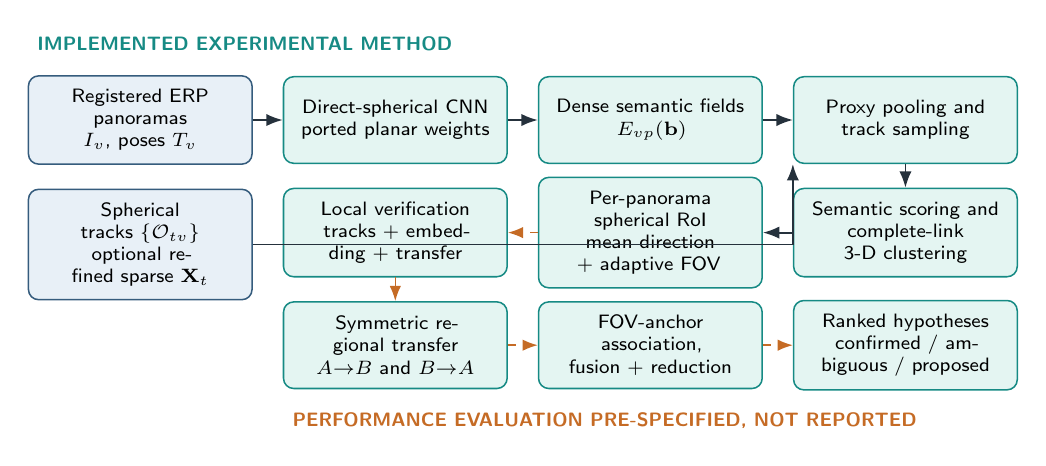
\begin{tikzpicture}[
  font=\sffamily\scriptsize,
  >=Latex,
  node distance=3.0mm and 3.8mm,
  stage/.style={rounded corners=1.3mm, draw=ink, line width=.55pt, minimum height=11mm, text width=25mm, align=center, inner sep=1.7mm},
  available/.style={stage, fill=evalfill, draw=eval},
  planned/.style={stage, fill=propfill, draw=prop},
  input/.style={stage, fill=inputfill, draw=inputblue},
  arrow/.style={->, line width=.65pt, draw=ink},
  soft/.style={->, line width=.55pt, dashed, draw=prop}
]
\node[input] (erp) {Registered ERP panoramas\\$I_v$, poses $T_v$};
\node[input, below=of erp] (tracks) {Spherical tracks $\{\mathcal O_{tv}\}$\\optional refined sparse $\mathbf X_t$};
\node[available, right=of erp] (scnn) {Direct-spherical CNN\\ported planar weights};
\node[available, right=of scnn] (cam) {Dense semantic fields\\$E_{vp}(\mathbf b)$};
\node[available, right=of cam] (sample) {Proxy pooling and\\track sampling};
\node[available, below=of sample] (cluster) {Semantic scoring and\\complete-link 3-D clustering};
\node[available, left=of cluster] (roi) {Per-panorama spherical RoI\\mean direction + adaptive FOV};
\node[available, left=of roi] (verify) {Local verification\\tracks + embedding + transfer};
\node[available, below=of verify] (transfer) {Symmetric regional transfer\\$A{\rightarrow}B$ and $B{\rightarrow}A$};
\node[available, right=of transfer] (reduce) {FOV-anchor association,\\fusion + reduction};
\node[available, right=of reduce] (output) {Ranked hypotheses\\confirmed / ambiguous / proposed};
\draw[arrow] (erp) -- (scnn);
\draw[arrow] (scnn) -- (cam);
\draw[arrow] (cam) -- (sample);
\draw[arrow] (tracks.east) -| (sample.south west);
\draw[arrow] (sample) -- (cluster);
\draw[arrow] (cluster) -- (roi);
\draw[soft] (roi) -- (verify);
\draw[soft] (verify) -- (transfer);
\draw[soft] (transfer) -- (reduce);
\draw[soft] (reduce) -- (output);
\node[anchor=west, font=\sffamily\scriptsize\bfseries, text=eval] at ([yshift=4mm]erp.north west) {IMPLEMENTED EXPERIMENTAL METHOD};
\node[anchor=west, font=\sffamily\scriptsize\bfseries, text=prop] at ([yshift=-4mm]transfer.south west) {PERFORMANCE EVALUATION PRE-SPECIFIED, NOT REPORTED};
\end{tikzpicture}
\caption{Method architecture. Teal stages are implemented as an Experimental, auditable pipeline. Semantic inference operates directly on the ERP sphere; gnomonic faces are transient local verification regions, not a multiface semantic inference path. The experimental programme evaluates the method but is intentionally not reported in this manuscript.}
\label{fig:pipeline}
\end{figure*}

\section{Related Work}

\subsection{Dense classification evidence}

Fully convolutional networks replace fixed-size fully connected operations by spatial operators, so larger inputs produce correspondingly denser outputs \citep{long2015fcn}. CAM expresses a class logit as a weighted sum of final convolutional channels \citep{zhou2016cam}. Its localization is weakly supervised: the map explains classification evidence, not object occupancy. The proposed method preserves that meaning and never converts a CAM threshold directly into ground truth.

Spherical CNNs address the position-dependent distortion created when a spherical signal is stored in a plane \citep{cohen2018spherical}. Our goal is not to train a new rotation-equivariant model. We port frozen planar filters to a differentiable geometry-aware sampler, retaining the learned vocabulary while changing how each kernel samples the sphere.

\subsection{Region proposals, masks, and reduction}

The R-CNN family established the two-stage pattern of generating candidates and then verifying or refining them \citep{girshick2014rcnn,girshick2015fast,ren2015faster}. Mask R-CNN showed that mask estimation can remain a separate branch attached to a region \citep{he2017mask}. Accordingly, SAM or another segmenter is optional in our pipeline and is invoked only if a boundary, area, or cutout is required.

Detector outputs are typically reduced by non-maximum suppression. Soft-NMS continuously decays a candidate score as overlap increases \citep{bodla2017softnms}; weighted boxes fusion averages compatible coordinates by confidence \citep{solovyev2021wbf}. We generalize those operations to regions on $\sphere$ and support in $\R^3$. Because two objects may overlap angularly while lying at different depths, spherical overlap alone is insufficient.

\section{Problem Definition}

Let $\mathcal V=\{1,\ldots,V\}$ index registered ERP panoramas $I_v$ of shape $(H_v,W_v)$. The registration of panorama $v$ consists of its camera centre $\mathbf C_v\in\R^3$ and world-to-panorama rotation $\mathbf R_v$. A feature track $t\in\mathcal T$ identifies image measurements believed to arise from the same physical point. The method does not require its precise 3-D position as input. If a successful geometric refinement already accepted a sparse landmark $\mathbf X_t$, that estimate is reused. Otherwise $\mathbf X_t$ is a latent variable estimated from the registered poses and the track bearings. In both cases $\mathbf X_t$ denotes an accepted sparse estimate, not ground truth or the physical object centre.

In typed form, $I_v\in\R^{H_v\times W_v\times3}$ is an RGB tensor,
$\mathbf C_v\in\R^3$ is a column vector in declared world units, and
$\mathbf R_v\in SO(3)\subset\R^{3\times3}$ is a rotation matrix. The product
$\mathbf R_v(\mathbf X-\mathbf C_v)$ is therefore a 3-vector in the panorama
camera frame. The indices $v$ and $t$ are integers; neither is a measured
quantity.

An observation of track $t$ in panorama $v$ is
\begin{equation}
 \mathcal O_{tv}=(v,\mathbf u_{tv},\mathbf b_{tv},r_{tv}),
 \qquad \mathbf b_{tv}=\mathbf b(\mathbf u_{tv})\in\sphere,
 \label{eq:trackobservation}
\end{equation}
where $\mathbf u_{tv}$ is the measured ERP feature location and $\mathbf b_{tv}$ is its measured unit bearing under the canonical pixel-centre map of Eqs.~\ref{eq:erpangles}--\ref{eq:erpray}. Independently, the reconstructed point predicts the unit bearing
\begin{equation}
 \widehat{\mathbf b}_{tv}=
 \frac{\mathbf R_v(\mathbf X_t-\mathbf C_v)}
 {\|\mathbf R_v(\mathbf X_t-\mathbf C_v)\|_2},\qquad
 r_{tv}=\cos^{-1}\!\left(
 \clip(\mathbf b_{tv}^{\top}\widehat{\mathbf b}_{tv},-1,1)
 \right).
 \label{eq:angularresidual}
\end{equation}
The observation $\mathcal O_{tv}$ is a heterogeneous record:
$v$ is an integer ID, $\mathbf u_{tv}\in\R^2$ is a two-coordinate image
measurement, $\mathbf b_{tv}\in\R^3$ is a unit vector, and
$r_{tv}\in\R$ is a scalar angle. In Eq.~\ref{eq:angularresidual}, the
subtraction and rotation produce a 3-vector, normalization produces a unit
3-vector, the dot product produces one cosine scalar, and $\cos^{-1}$ converts
that scalar to an angle. The clip is a numerical guard against round-off just
outside $[-1,1]$.
The pixel and its bearing are measurement-derived fields; $r_{tv}$ is a
diagnostic field populated only after a candidate $\mathbf X_t$ is available.
It must not be mistaken for a fourth raw sensor measurement.
Thus $r_{tv}\in[0,\pi]$ is the geodesic angle, in radians, between the direction actually measured in the panorama and the direction predicted by $\mathbf X_t$. It is zero only under exact reprojection; a threshold on $r_{tv}$ rejects geometrically inconsistent track observations. Low parallax or an ill-conditioned intersection is a local track degeneracy. In contrast, systematic cheirality or reprojection failure across non-degenerate tracks is treated as evidence that the supplied $(\mathbf R_v,\mathbf C_v)$, equivalently $(\mathbf R_v,\mathbf t_v)$, are inconsistent; the method then stops instead of manufacturing bearing-only spatial support.

Geometric observation and semantic evidence are separate records keyed by the same panorama ID $v$. Semantic inference augments the registered panorama; it does not create a second camera, a second ``view'', or a stored gnomonic face. Let $\mathcal V_E\subseteq\mathcal V$ contain exactly the panorama IDs with semantic evidence. For $v\in\mathcal V_E$, the attached evidence record is
\begin{equation}
 \mathcal D_v=
 \left(v,\{E_{vp}\}_{p\in\mathcal L_v},
 Q_v,\nu_v,\pi_v\right),\qquad v\in\mathcal V_E,
 \label{eq:evidencerecord}
\end{equation}
where $\mathcal L_v$ is the channel-label set, $\nu_v$ identifies the frozen vocabulary/model contract, and $\pi_v$ stores provenance. We call the pair $(I_v,\mathcal D_v)$ an \emph{evidence-bearing panorama}. Throughout the paper, \emph{view} refers only to the original registered panorama and camera; $\mathcal D_v$ is an attachment to it, not another observation.

Each evidence record contains dense directional channels and explicit support:
\begin{equation}
 E_{vp}:\sphere\rightarrow[0,1],\qquad
 Q_v:\sphere\rightarrow\{0,1\},
 \label{eq:evidence}
\end{equation}
where $p$ is an exact classifier label or fixed proxy. A zero score is valid evidence and is never inferred to mean invalid data. A concept $c$ is declared before evaluation by proxy set $\mathcal P_c$ and positive normalized weights $a_{cp}$, $\sum_p a_{cp}=1$.

The output hypothesis is
\begin{equation}
 \mathcal H_i=(c_i,q_i,\mathcal T_i,\mathcal V_i,
 \mathcal S_i,\mathcal G_i,\mathcal P_i,\eta_i),
 \label{eq:hypothesis}
\end{equation}
where $c_i$ is the declared concept, $q_i\in[0,1]$ is its aggregate confidence, $\mathcal T_i\subseteq\mathcal T$ contains the supporting track IDs, $\mathcal V_i\subseteq\mathcal V_E$ contains the supporting panorama IDs, $\mathcal G_i=\{R_{iv}:v\in\mathcal V_i\}$ contains the per-panorama spherical regions, $\mathcal P_i$ records model, vocabulary, geometry, and reduction provenance, and $\eta_i\in\{\text{proposed},\text{ambiguous},\text{confirmed}\}$ is the decision state. Spatial support is a tagged object
\begin{equation}
 \mathcal S_i=
 \begin{cases}
  (\kappa_i,\bm\mu_i,\bm\Sigma_i,\rho_i),
   & \kappa_i\in\{\text{metric},\text{scale-free}\},\\
  (\text{bearing-only},\varnothing),
   & \text{if no reconstructed point supports }i,
 \end{cases}
 \label{eq:spatialsupport}
\end{equation}
where the first case summarizes finite 3-D support in declared world units and the second leaves directional extent exclusively in $\mathcal G_i$. Thus unsupported semantic evidence can never silently acquire a 3-D position.

Equation~\ref{eq:hypothesis} should be read as a schema, not as concatenation
into one vector. Its fields have different types: $c_i$ and $\eta_i$ are
categorical values, $q_i$ is a scalar, $\mathcal T_i$ and $\mathcal V_i$ are
sets of IDs, $\mathcal S_i$ is a tagged spatial record, $\mathcal G_i$ is a
set of region records, and $\mathcal P_i$ is provenance. In the finite-support
case, $\bm\mu_i\in\R^3$, $\bm\Sigma_i\in\R^{3\times3}$, and
$\rho_i\in\R_{\ge0}$. In the bearing-only case, those quantities are absent
rather than filled with zero, preventing ``unknown position'' from being
mistaken for the world origin.

\begin{figure*}[t]
\centering
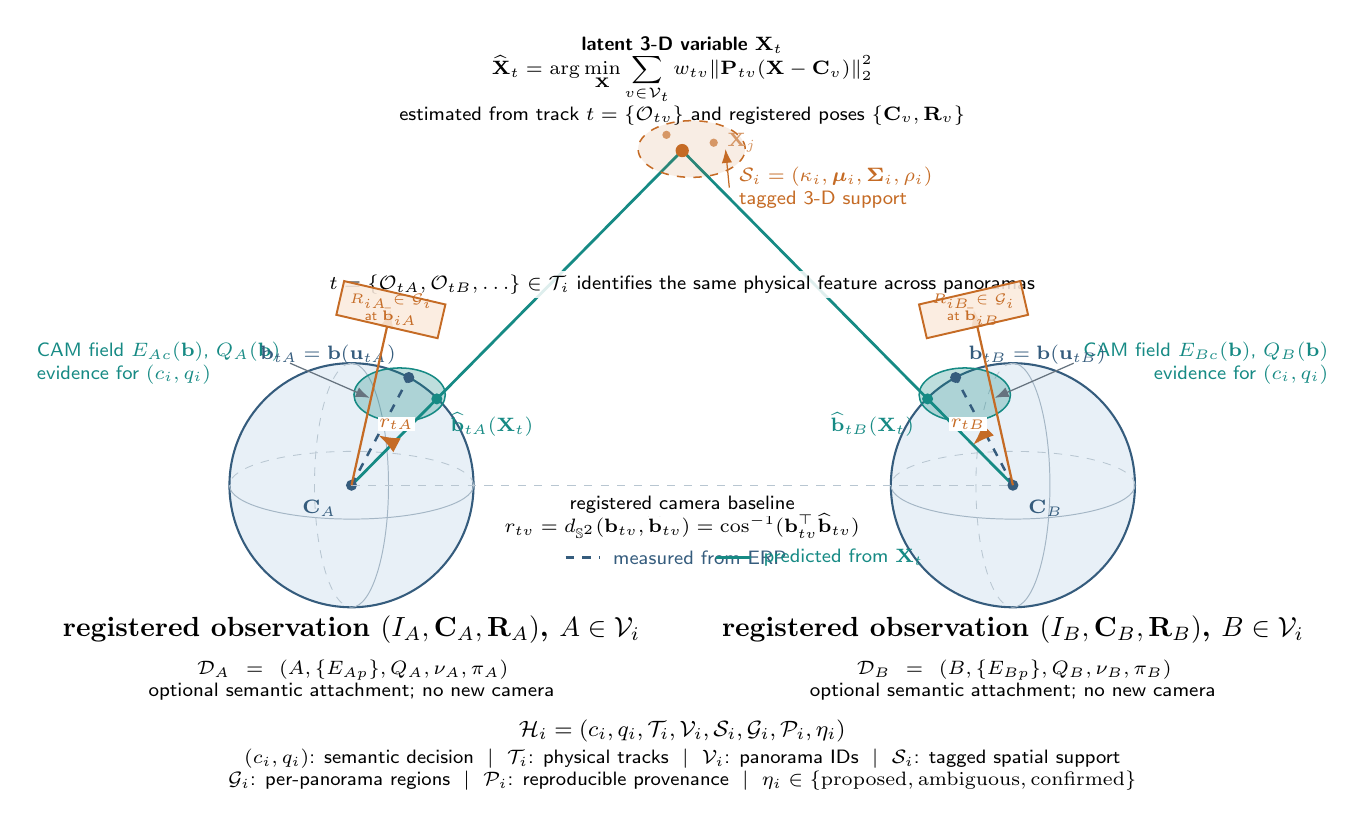
\begin{tikzpicture}[
  font=\sffamily\scriptsize,
  >=Latex,
  sphere/.style={draw=inputblue,line width=.75pt,fill=inputfill},
  grid/.style={draw=inputblue!45,line width=.35pt},
  hidden/.style={draw=inputblue!35,dashed,line width=.3pt},
  track/.style={draw=eval,line width=1.0pt},
  meanray/.style={->,draw=prop,line width=.8pt},
  plane/.style={draw=prop,line width=.7pt,fill=propfill,fill opacity=.88},
  callout/.style={->,draw=muted,line width=.45pt}
]
\coordinate (ca) at (0,0);
\coordinate (cb) at (8.4,0);
\coordinate (xt) at (4.2,4.25);
\coordinate (bha) at ($(ca)!.258!(xt)$);
\coordinate (bhb) at ($(cb)!.258!(xt)$);
\coordinate (ba) at ([shift={(62:1.55cm)}]ca);
\coordinate (bb) at ([shift={(118:1.55cm)}]cb);
\coordinate (eac) at ($(ca)!.84!(ba)$);
\coordinate (ebc) at ($(cb)!.84!(bb)$);

% The two registered omnidirectional observations, represented as viewing
% spheres rather than as image boxes.
\draw[sphere] (ca) circle (1.55);
\draw[grid] ([xshift=-1.55cm]ca) arc[start angle=180,end angle=360,x radius=1.55cm,y radius=.43cm];
\draw[hidden] ([xshift=1.55cm]ca) arc[start angle=0,end angle=180,x radius=1.55cm,y radius=.43cm];
\draw[grid] ([yshift=-1.55cm]ca) arc[start angle=-90,end angle=90,x radius=.47cm,y radius=1.55cm];
\draw[hidden] ([yshift=1.55cm]ca) arc[start angle=90,end angle=270,x radius=.47cm,y radius=1.55cm];
\node[font=\bfseries] at ($(ca)+(0,-1.83)$) {registered observation $(I_A,\mathbf C_A,\mathbf R_A)$, $A\in\mathcal V_i$};

\draw[sphere] (cb) circle (1.55);
\draw[grid] ([xshift=-1.55cm]cb) arc[start angle=180,end angle=360,x radius=1.55cm,y radius=.43cm];
\draw[hidden] ([xshift=1.55cm]cb) arc[start angle=0,end angle=180,x radius=1.55cm,y radius=.43cm];
\draw[grid] ([yshift=-1.55cm]cb) arc[start angle=-90,end angle=90,x radius=.47cm,y radius=1.55cm];
\draw[hidden] ([yshift=1.55cm]cb) arc[start angle=90,end angle=270,x radius=.47cm,y radius=1.55cm];
\node[font=\bfseries] at ($(cb)+(0,-1.83)$) {registered observation $(I_B,\mathbf C_B,\mathbf R_B)$, $B\in\mathcal V_i$};

% Class evidence is a field on each sphere, not an object mask.
\fill[eval,opacity=.28] (eac) ellipse (.58 and .34);
\draw[eval,line width=.55pt] (eac) ellipse (.58 and .34);
\fill[eval,opacity=.28] (ebc) ellipse (.58 and .34);
\draw[eval,line width=.55pt] (ebc) ellipse (.58 and .34);
\node[eval,align=left] (ea) at (-2.45,1.55) {CAM field $E_{Ac}(\mathbf b)$, $Q_A(\mathbf b)$\\evidence for $(c_i,q_i)$};
\draw[callout] (ea.east)--($(eac)+(-.38,-.04)$);
\node[eval,align=right] (eb) at (10.85,1.55) {CAM field $E_{Bc}(\mathbf b)$, $Q_B(\mathbf b)$\\evidence for $(c_i,q_i)$};
\draw[callout] (eb.west)--($(ebc)+(.38,-.04)$);

% The solid rays are predictions from X_t. Dashed rays are the measured ERP
% bearings; their geodesic separation is the angular reprojection residual.
\draw[track] (ca)--(xt);
\draw[track] (cb)--(xt);
\draw[draw=inputblue,dashed,line width=.9pt] (ca)--(ba);
\draw[draw=inputblue,dashed,line width=.9pt] (cb)--(bb);
\draw[->,draw=prop,line width=1.05pt] ($(ca)+(45.3:.72)$)
 arc[start angle=45.3,end angle=62,radius=.72];
\node[prop,fill=white,inner sep=.5pt] at ($(ca)+(53.6:.96)$) {$r_{tA}$};
\draw[->,draw=prop,line width=1.05pt] ($(cb)+(118:.72)$)
 arc[start angle=118,end angle=134.7,radius=.72];
\node[prop,fill=white,inner sep=.5pt] at ($(cb)+(126.4:.96)$) {$r_{tB}$};
\fill[inputblue] (ca) circle (2.0pt) node[below left=1mm] {$\mathbf C_A$};
\fill[inputblue] (cb) circle (2.0pt) node[below right=1mm] {$\mathbf C_B$};
\fill[inputblue] (ba) circle (2.0pt) node[above left=.6mm] {$\mathbf b_{tA}=\mathbf b(\mathbf u_{tA})$};
\fill[inputblue] (bb) circle (2.0pt) node[above right=.6mm] {$\mathbf b_{tB}=\mathbf b(\mathbf u_{tB})$};
\fill[eval] (bha) circle (2.0pt) node[below right=.7mm] {$\widehat{\mathbf b}_{tA}(\mathbf X_t)$};
\fill[eval] (bhb) circle (2.0pt) node[below left=.7mm] {$\widehat{\mathbf b}_{tB}(\mathbf X_t)$};
\fill[prop,opacity=.12] ($(xt)+(.12,.02)$) ellipse (.68 and .36);
\draw[prop,dashed,line width=.55pt] ($(xt)+(.12,.02)$) ellipse (.68 and .36);
\fill[prop!70] ($(xt)+(.40,.10)$) circle (1.5pt) node[right=.5mm] {$\mathbf X_j$};
\fill[prop!70] ($(xt)+(-.20,.20)$) circle (1.5pt);
\fill[prop] (xt) circle (2.4pt);
\node[above=2mm of xt,align=center] {
 \textbf{latent 3-D variable $\mathbf X_t$}\\[-.2mm]
 $\displaystyle \widehat{\mathbf X}_t=\arg\min_{\mathbf X}
 \sum_{v\in\mathcal V_t}w_{tv}
 \|\mathbf P_{tv}(\mathbf X-\mathbf C_v)\|_2^2$\\[-.2mm]
 estimated from track $t=\{\mathcal O_{tv}\}$ and registered poses
 $\{\mathbf C_v,\mathbf R_v\}$};
\node[prop,align=left] (si) at (6.15,3.78) {$\mathcal S_i=(\kappa_i,\bm\mu_i,\bm\Sigma_i,\rho_i)$\\tagged 3-D support};
\draw[callout,draw=prop] (si.west)--($(xt)+(.55,.02)$);
\node[align=center,fill=white,fill opacity=.86,text opacity=1,inner sep=1.5pt] at (4.2,2.55)
 {$t=\{\mathcal O_{tA},\mathcal O_{tB},\ldots\}\in\mathcal T_i$
 identifies the same physical feature across panoramas};
\node[align=center,font=\sffamily\scriptsize] at (4.2,-.52)
 {$r_{tv}=d_{\sphere}(\mathbf b_{tv},\widehat{\mathbf b}_{tv})
 =\cos^{-1}(\mathbf b_{tv}^{\top}\widehat{\mathbf b}_{tv})$};
\draw[inputblue,dashed,line width=.9pt] (2.72,-.92)--(3.16,-.92);
\node[anchor=west,text=inputblue] at (3.20,-.92) {measured from ERP};
\draw[eval,line width=1.0pt] (4.63,-.92)--(5.07,-.92);
\node[anchor=west,text=eval] at (5.11,-.92) {predicted from $\mathbf X_t$};
\draw[hidden] (ca)--(cb) node[midway,below=1mm,fill=white,inner sep=1pt] {registered camera baseline};

% The mean supported direction opens one transient tangent-plane crop per
% panorama; it does not introduce another camera observation.
\draw[meanray] (ca)--(.50,2.23);
\begin{scope}[shift={(.50,2.23)},rotate=167]
  \draw[plane] (-.66,-.22) rectangle (.66,.22);
\end{scope}
\node[prop,align=center,font=\sffamily\tiny] at (.50,2.23) {$R_{iA}\in\mathcal G_i$\\at $\bar{\mathbf b}_{iA}$};

\draw[meanray] (cb)--(7.90,2.23);
\begin{scope}[shift={(7.90,2.23)},rotate=13]
  \draw[plane] (-.66,-.22) rectangle (.66,.22);
\end{scope}
\node[prop,align=center,font=\sffamily\tiny] at (7.90,2.23) {$R_{iB}\in\mathcal G_i$\\at $\bar{\mathbf b}_{iB}$};

% Evidence records remain attached to the original panorama IDs.
\node[align=center,text width=55mm] at ($(ca)+(0,-2.48)$)
 {$\mathcal D_A=(A,\{E_{Ap}\},Q_A,\nu_A,\pi_A)$\\optional semantic attachment; no new camera};
\node[align=center,text width=55mm] at ($(cb)+(0,-2.48)$)
 {$\mathcal D_B=(B,\{E_{Bp}\},Q_B,\nu_B,\pi_B)$\\optional semantic attachment; no new camera};

\node[align=center,font=\sffamily\footnotesize] at (4.2,-3.12)
 {$\displaystyle \mathcal H_i=
 (c_i,q_i,\mathcal T_i,\mathcal V_i,\mathcal S_i,
 \mathcal G_i,\mathcal P_i,\eta_i)$};
\node[align=center,font=\sffamily\scriptsize] at (4.2,-3.47)
 {$(c_i,q_i)$: semantic decision $\;\mid\;$
 $\mathcal T_i$: physical tracks $\;\mid\;$
 $\mathcal V_i$: panorama IDs $\;\mid\;$
 $\mathcal S_i$: tagged spatial support};
\node[align=center,font=\sffamily\scriptsize] at (4.2,-3.75)
 {$\mathcal G_i$: per-panorama regions $\;\mid\;$
 $\mathcal P_i$: reproducible provenance $\;\mid\;$
 $\eta_i\in\{\mathrm{proposed},\mathrm{ambiguous},\mathrm{confirmed}\}$};
\end{tikzpicture}
\caption{Geometric reading of the observation and hypothesis definitions. For each panorama, the dashed ray is the bearing $\mathbf b_{tv}=\mathbf b(\mathbf u_{tv})$ measured from the matched ERP feature. The solid ray is the bearing $\widehat{\mathbf b}_{tv}$ predicted by projecting the accepted sparse estimate $\mathbf X_t$ through $(\mathbf C_v,\mathbf R_v)$. The point may come from a successful prior refinement or be estimated here from the registered rays; it is never assumed precise. Their geodesic separation is the angular reprojection residual $r_{tv}$; the arcs are exaggerated for legibility. Solid rays from both cameras meet at $\mathbf X_t$, whereas measured rays need not meet it exactly. Teal surface patches are CAM evidence fields, not masks. The original registered observations supply $\mathcal V_i$ and $\mathcal T_i$; neighbouring accepted track points form $\mathcal S_i$; tangent regions form $\mathcal G_i$; attached evidence records contribute $\mathcal P_i$ without creating new cameras; and the acceptance logic assigns $\eta_i$.}
\label{fig:problem}
\end{figure*}

\section{Method}

\subsection{How to read the mathematics}

The notation distinguishes a number from a direction, a coordinate transform,
a sampled image, and a logical collection. Plain lower-case symbols such as
$s$, $q$, $r$, $\lambda$, and $\varphi$ are \emph{scalars}: each stores one
real number. Bold lower-case symbols such as $\mathbf b$ are column
\emph{vectors}; bold upper-case symbols such as $\mathbf R$ are
\emph{matrices}. An image or feature lattice is an indexed \emph{tensor}, a
calligraphic symbol such as $\mathcal T$ is a set or structured record, and a
map such as $E:\sphere\rightarrow[0,1]$ is a continuous-domain field that is
stored numerically on a discrete lattice. The same letter is never intended to
switch type within an equation.

Indices also have fixed roles: $v$ identifies a registered panorama, $t$ a
feature track, $p$ an exact model label, $c$ a declared semantic concept, $i$
a hypothesis, and $k$ a feature channel. Superscript $\top$ transposes a
vector or matrix, $\|\cdot\|_2$ is Euclidean length, $\mathbf a^\top\mathbf b$
is a scalar dot product, and $\mathbf a\mathbf a^\top$ is a matrix outer
product. Table~\ref{tab:types} is a compact type reference used throughout the
method.

\begin{table*}[t]
\centering
\caption{Typed notation. Shapes are mathematical shapes, independent of a particular array layout in software. Angles are real scalars measured in radians.}
\label{tab:types}
\begin{tabular}{@{}p{25mm}p{42mm}p{88mm}@{}}
\toprule
Symbol & Type and shape & Meaning and a concrete reading\\
\midrule
$x,y,H,W,$\newline $v,t,p,c,i,k$ & integer scalars in $\mathbb Z$ & Pixel coordinates, dimensions, or discrete identifiers. For example, $v=3$ selects one registered panorama.\\
$s,q,r,\lambda,\varphi,\theta$ & real scalars in $\R$ & A score, confidence, residual, longitude, latitude, or field of view. One scalar has no spatial direction by itself.\\
$\mathbf u$ & vector in $\R^2$ & A two-coordinate ERP location, e.g. $\mathbf u=(x,y)^\top$.\\
$\mathbf b,\mathbf d,\mathbf C,\mathbf X,\bm\mu$ & vectors in $\R^3$ & Directions and points. Unit bearings satisfy $\|\mathbf b\|_2=1$; camera centres and 3-D points additionally carry declared units.\\
$\mathbf R$ & matrix in $SO(3)\subset\R^{3\times3}$ & A rotation: multiplying $\mathbf R\mathbf X$ maps one 3-vector into another frame without changing its length.\\
$\mathbf P,\mathbf A,\bm\Sigma$ & matrices in $\R^{3\times3}$ & Respectively a ray-orthogonal projector, a least-squares system matrix, and a spatial second-moment matrix.\\
$I_v$; $A_v$ & tensors in $\R^{H_v\times W_v\times3}$; $\R^{H_L\times W_L\times K}$ & An RGB panorama and a $K$-channel convolutional feature lattice. A location in $A_v$ stores a vector in $\R^K$.\\
$E_{vp}$; $Q_v$ & fields $\sphere\to[0,1]$; $\sphere\to\{0,1\}$ & Class evidence and explicit validity. $E=0$ is a valid low score; only $Q=0$ means unsupported.\\
$\mathcal V,\mathcal T,\mathcal P_c,K_i$ & finite sets & Panorama IDs, track IDs, proxy labels, and the tracks assigned to a cluster. Set intersection and union act on IDs, not pixel values.\\
$\mathcal O,\mathcal D,\mathcal H,R_{iv}$ & structured records & An observation, evidence attachment, output hypothesis, and per-panorama spherical region. A record groups typed values but is not itself a numeric vector.\\
\bottomrule
\end{tabular}
\end{table*}

Figure~\ref{fig:typedflow} shows where these types change. Geometry converts a
2-D measurement into a 3-D unit direction and, across views, into an estimated
3-D point. Semantics converts an RGB tensor into a feature vector and then into
a scalar evidence field. The two branches meet only by sampling the semantic
field at a registered bearing. That sampled scalar annotates a geometric track;
it does not alter the track position.

\begin{figure*}[t]
\centering
\resizebox{\textwidth}{!}{%
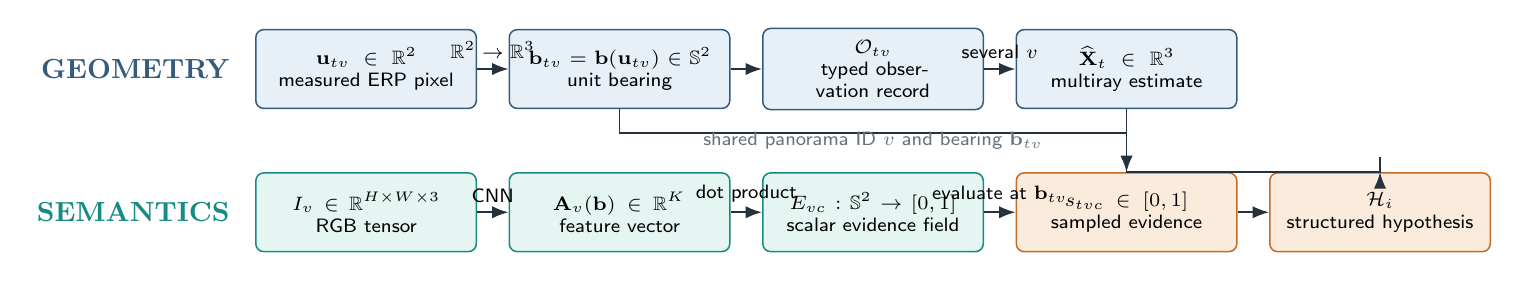
\begin{tikzpicture}[
 font=\sffamily\scriptsize,>=Latex,
 box/.style={rounded corners=1mm,draw=ink,line width=.55pt,minimum height=10mm,text width=25mm,align=center,inner sep=1.5mm},
 geo/.style={box,fill=inputfill,draw=inputblue},
 sem/.style={box,fill=evalfill,draw=eval},
 result/.style={box,fill=propfill,draw=prop},
 arr/.style={->,draw=ink,line width=.65pt}
]
\node[geo] (pixel) {$\mathbf u_{tv}\in\R^2$\\measured ERP pixel};
\node[geo,right=4mm of pixel] (bearing) {$\mathbf b_{tv}=\mathbf b(\mathbf u_{tv})\in\sphere$\\unit bearing};
\node[geo,right=4mm of bearing] (obs) {$\mathcal O_{tv}$\\typed observation record};
\node[geo,right=4mm of obs] (point) {$\widehat{\mathbf X}_t\in\R^3$\\multiray estimate};
\node[sem,below=8mm of pixel] (image) {$I_v\in\R^{H\times W\times3}$\\RGB tensor};
\node[sem,right=4mm of image] (features) {$\mathbf A_v(\mathbf b)\in\R^K$\\feature vector};
\node[sem,right=4mm of features] (field) {$E_{vc}:\sphere\to[0,1]$\\scalar evidence field};
\node[result,right=4mm of field] (sample) {$s_{tvc}\in[0,1]$\\sampled evidence};
\node[result,right=4mm of sample] (hyp) {$\mathcal H_i$\\structured hypothesis};
\draw[arr] (pixel)-- node[above] {$\R^2\to\R^3$} (bearing);
\draw[arr] (bearing)--(obs);
\draw[arr] (obs)-- node[above] {several $v$} (point);
\draw[arr] (image)-- node[above] {CNN} (features);
\draw[arr] (features)-- node[above] {dot product} (field);
\draw[arr] (field)-- node[above] {evaluate at $\mathbf b_{tv}$} (sample);
\draw[arr] (bearing.south)--++(0,-3mm)-|(sample.north);
\draw[arr] (point.south)--++(0,-8mm)-|(hyp.north);
\draw[arr] (sample)--(hyp);
\node[anchor=east,text=inputblue,font=\bfseries] at ([xshift=-2mm]pixel.west) {GEOMETRY};
\node[anchor=east,text=eval,font=\bfseries] at ([xshift=-2mm]image.west) {SEMANTICS};
\node[align=center,text=muted] at ($(obs)!0.5!(field)$) {shared panorama ID $v$ and bearing $\mathbf b_{tv}$};
\end{tikzpicture}
}
\caption{Typed data flow. Arrows state operations, while boxes state the resulting data type. The geometric and semantic branches remain independent until a scalar field is evaluated at a registered bearing. The final hypothesis groups sets, scalars, vectors, matrices, regions, and provenance; it is not a single feature vector.}
\label{fig:typedflow}
\end{figure*}

\subsection{Canonical spherical geometry}

We use pixel centres, top-left image origin, $+X$ right, $+Y$ up, and $+Z$ forward. An ERP pixel $(x,y)$ maps to
\begin{align}
 \lambda &=2\pi\frac{x+1/2}{W}-\pi, &
 \varphi &=\frac{\pi}{2}-\pi\frac{y+1/2}{H}, \label{eq:erpangles}\\
 \mathbf b(x,y)&=(\sin\lambda\cos\varphi,
 \sin\varphi,\cos\lambda\cos\varphi). \label{eq:erpray}
\end{align}
Longitude is periodic in $[-\pi,\pi)$ and latitude decreases north-to-south. These conventions govern semantic sampling, feature bearings, projection, masks, and solid-angle evaluation.

Here $x,y,H,W$ are integer scalars, $\lambda$ and $\varphi$ are real
scalars in radians, and $\mathbf b$ is a three-component column vector. The
trigonometric expression constructs the vector component by component; it does
not multiply a matrix. For example, the ideal ERP centre
$x+1/2=W/2$, $y+1/2=H/2$ gives
$(\lambda,\varphi)=(0,0)$ and therefore
$\mathbf b=(0,0,1)^\top$, the forward direction. The first and last ERP
columns approach the same meridian from opposite sides, so horizontal sampling
must wrap rather than pad with invalid pixels. Substitution into
Eq.~\ref{eq:erpray} gives $\|\mathbf b\|_2=1$, which is the dimensional check
used before any angular operation.

\subsection{Sparse support from poses and bearing tracks}

The geometric input is a set of registered poses and cross-view bearing tracks; an exact $\mathbf X_t$ is not required. If pose is supplied as $\mathbf x_v=\mathbf R_v\mathbf X+\mathbf t_v$, then $\mathbf C_v=-\mathbf R_v^\top\mathbf t_v$ and the world-frame ray direction is
\begin{equation}
 \mathbf d_{tv}=\mathbf R_v^\top\mathbf b_{tv},\qquad
 \mathbf P_{tv}=\mathbf I-\mathbf d_{tv}\mathbf d_{tv}^\top.
 \label{eq:worldray}
\end{equation}
With declared positive observation weights $w_{tv}$, the latent sparse point is estimated by multiray least squares,
\begin{equation}
 \widehat{\mathbf X}_t=\mathbf A_t^\dagger\mathbf y_t,\qquad
 \mathbf A_t=\sum_v w_{tv}\mathbf P_{tv},\qquad
 \mathbf y_t=\sum_v w_{tv}\mathbf P_{tv}\mathbf C_v.
 \label{eq:multiray}
\end{equation}
The types make the least-squares construction explicit. Both
$\mathbf d_{tv}$ and $\mathbf C_v$ are 3-vectors. The outer product
$\mathbf d_{tv}\mathbf d_{tv}^{\top}$ is a $3\times3$ matrix, so
$\mathbf P_{tv}\in\R^{3\times3}$. Multiplying this matrix by a point produces
a 3-vector: $\mathbf P_{tv}\mathbf C_v\in\R^3$. Consequently
$\mathbf A_t\in\R^{3\times3}$, $\mathbf y_t\in\R^3$, and the pseudoinverse
$\mathbf A_t^\dagger\in\R^{3\times3}$ returns
$\widehat{\mathbf X}_t\in\R^3$.

Geometrically, $\mathbf P_{tv}$ deletes the component parallel to the ray:
$\mathbf P_{tv}\mathbf d_{tv}=\mathbf0$. Therefore
$\|\mathbf P_{tv}(\mathbf X-\mathbf C_v)\|_2$ is the perpendicular distance
from a trial point $\mathbf X$ to the infinite line supporting ray $(v,t)$.
Equation~\ref{eq:multiray}
minimizes the weighted sum of these squared perpendicular distances. With two
well-separated rays, it selects the point nearest both rays; with nearly
parallel rays, $\mathbf A_t$ becomes ill-conditioned and the method explicitly
abstains. A separate positive-depth test then enforces the ray, rather than
line, interpretation. Figure~\ref{fig:problem} visualizes measured bearings, predicted
bearings, the latent 3-D variable, and the residual angles.
When a previous geometric refinement already supplies a valid sparse $\mathbf X_t$, the method reuses it instead of recomputing Eq.~\ref{eq:multiray}, but applies the same cheirality and angular-residual checks. This is a provenance requirement: a point sampled from depth, scanner XYZ, or a one-shot reprojection filter is not relabelled as a refined visual landmark. Without post-refinement inliers, the coordinate is discarded and Eq.~\ref{eq:multiray} is evaluated from poses and measured bearings. The notation $\mathbf X_t$ below means whichever accepted sparse estimate is used.

For an internally estimated point, let $\alpha_t$ be the maximum pairwise angle between its world rays and $\kappa_t=\operatorname{cond}(\mathbf A_t)$. A track is locally degenerate when $\alpha_t<\tau_\alpha$ or $\kappa_t>\tau_\kappa$; it contributes no finite support. A non-degenerate track is rejected when the positive-depth fraction is below $\tau_z$ or $\max_v r_{tv}>\tau_r$. Finally, let $\mathcal N$ be the non-degenerate tracks and $\mathcal R\subseteq\mathcal N$ those rejected by cheirality or reprojection. The registered geometry fails closed when
\begin{equation}
 |\mathcal N|\ge N_{\min}
 \quad\wedge\quad
 \frac{|\mathcal R|}{|\mathcal N|}>\tau_{\rm pose}.
 \label{eq:posegate}
\end{equation}
This separates an isolated weak-baseline feature from systematic evidence that $(\mathbf R,\mathbf t)$ is wrong. The latter cannot be hidden by emitting bearing-only object hypotheses.

All quantities in Eq.~\ref{eq:posegate} are scalars: $|\mathcal N|$ and
$|\mathcal R|$ are integer set cardinalities, their ratio is a real fraction,
and the comparisons return Boolean values. The conjunction $\wedge$ is a
logical operation, not multiplication. A failed pose gate stops the method,
whereas one degenerate track merely loses finite 3-D support.

\subsection{Direct-spherical convolution}

For location $\mathbf z\in\sphere$, a geometry-aware convolution samples a local tangent stencil instead of translating a kernel in ERP pixels:
\begin{equation}
 Y_o(\mathbf z)=\sum_i\sum_{\delta\in\mathcal K}
 W_{oi}(\delta)\,
 \widetilde X_i\!\left(q(\mathbf z,\delta)\right).
 \label{eq:sconv}
\end{equation}
$W$ is a frozen planar kernel, $q(\mathbf z,\delta)$ maps tangent offset $\delta$ to an ERP coordinate through the local spherical frame, and $\widetilde X$ denotes differentiable bilinear sampling with horizontal wrap. Learned weights are preserved; only the sampling lattice changes.
Formally, $\delta\in\mathcal K\subset\R^2$ is a two-component tangent offset
and $q:\sphere\times\R^2\rightarrow\R^2$ returns a two-component continuous
ERP coordinate. The map is geometric; it has no learned parameters.

More explicitly, let
$X\in\R^{C_{\rm in}\times H\times W}$,
$W\in\R^{C_{\rm out}\times C_{\rm in}\times K_h\times K_w}$, and
$Y\in\R^{C_{\rm out}\times H'\times W'}$. At one output location $\mathbf z$ and
channel $o$, $Y_o(\mathbf z)$ is a scalar. Each
$W_{oi}(\delta)$ is also a scalar, and
$\widetilde X_i(q(\mathbf z,\delta))$ is the scalar obtained by bilinearly sampling
input channel $i$ at a generally non-integer 2-D ERP coordinate. Their products
are summed over $C_{\rm in}K_hK_w$ terms. For a $3\times3$ kernel, nine tangent
offsets are sampled per input channel. Figure~\ref{fig:sconvtypes} contrasts
the fixed weight indices with their position-dependent spherical sample
coordinates.

\begin{figure}[t]
\centering
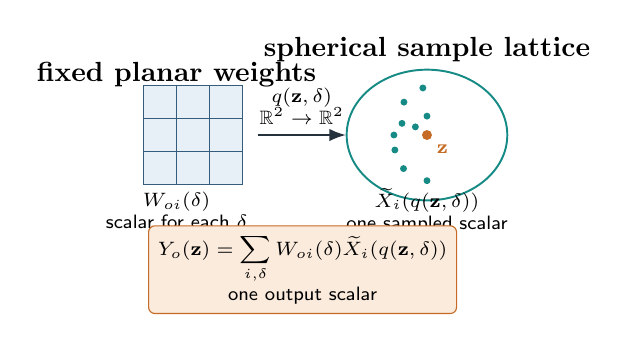
\begin{tikzpicture}[font=\sffamily\scriptsize,>=Latex]
\node[align=center,font=\bfseries] at (0,1.63) {fixed planar weights};
\foreach \x in {-1,0,1}{\foreach \y in {-1,0,1}{
  \draw[fill=inputfill,draw=inputblue]
    ($(0,0.65)+(\x*.42,\y*.42)$) rectangle ++(.42,.42);
}}
\node[align=center] at (0,-.10) {$W_{oi}(\delta)$\\scalar for each $\delta$};
\draw[->,draw=ink,line width=.65pt] (1.03,.86)--
 node[above,align=center] {$q(\mathbf z,\delta)$\\$\R^2\to\R^2$} (2.15,.86);
\draw[draw=eval,line width=.7pt] (3.18,.86) ellipse (1.02 and .83);
\foreach \a/\b in {155/.35,125/.51,95/.60,180/.42,145/.18,90/.24,205/.45,235/.52,270/.58}{
  \fill[eval] ($(3.18,.86)+(\a:\b)$) circle (1.25pt);
}
\fill[prop] (3.18,.86) circle (1.8pt) node[below right] {$\mathbf z$};
\node[align=center,font=\bfseries] at (3.18,1.95) {spherical sample lattice};
\node[align=center] at (3.18,-.10)
 {$\widetilde X_i(q(\mathbf z,\delta))$\\one sampled scalar};
\node[rounded corners=.8mm,draw=prop,fill=propfill,align=center]
 at (1.60,-.85)
 {$\displaystyle Y_o(\mathbf z)=\sum_{i,\delta}W_{oi}(\delta)\widetilde X_i(q(\mathbf z,\delta))$\\one output scalar};
\end{tikzpicture}
\caption{Typed spherical-convolution operation. The learned scalar weights and channel indices are unchanged. Only the coordinate $q(\mathbf z,\delta)$ used to sample each input scalar depends on spherical location $\mathbf z$.}
\label{fig:sconvtypes}
\end{figure}

For a network with total stride $s$, an input ERP of shape $(H,W)$ produces a native feature lattice approximately
\begin{equation}
 H_L=\left\lceil\frac{H}{s}\right\rceil,\qquad
 W_L=\left\lceil\frac{W}{s}\right\rceil.
 \label{eq:density}
\end{equation}
This is central to the experiment: increasing ERP resolution should increase native CAM density rather than forcing the panorama back to the classifier's nominal crop size.

For example, a stride-$32$ backbone evaluated at $1024\times2048$ produces an
approximately $32\times64$ native lattice, while the same fully convolutional
backbone evaluated at $2048\times4096$ produces approximately $64\times128$.
The number of spatial evidence samples grows fourfold. Upsampling a
$32\times64$ CAM to a larger display does not create the missing evidence; the
density gain must occur inside the network by evaluating the larger ERP.

\subsection{CAM and semantic proxy fields}

Let $A_{vk}(\mathbf b)$ be final feature channel $k$ at bearing $\mathbf b$ and $w_{pk}$ the frozen classifier weight for proxy class $p$. The non-negative CAM is
\begin{equation}
 \widehat E_{vp}(\mathbf b)=
 \left[\sum_k w_{pk}A_{vk}(\mathbf b)\right]_+.
 \label{eq:camraw}
\end{equation}
At one spherical location, collect the channels as
$\mathbf A_v(\mathbf b)=(A_{v1}(\mathbf b),\ldots,A_{vK}(\mathbf b))^\top\in\R^K$ and the classifier
row as $\mathbf w_p=(w_{p1},\ldots,w_{pK})^\top\in\R^K$. The sum in
Eq.~\ref{eq:camraw} is the dot product
$\mathbf w_p^\top\mathbf A_v(\mathbf b)\in\R$: two $K$-vectors produce one scalar.
The bracket $[z]_+=\max(z,0)$ is a scalar rectifier. As a small arithmetic
example, $\mathbf w=(0.5,-0.2,0.1)^\top$ and
$\mathbf A=(2,1,4)^\top$ give
$[\mathbf w^\top\mathbf A]_+=[1.0-0.2+0.4]_+=1.2$.
We normalize only over supported samples:
\begin{equation}
 E_{vp}(\mathbf b)=
 \frac{\widehat E_{vp}(\mathbf b)-m_{vp}}
 {M_{vp}-m_{vp}+\epsilon}, \quad Q_v(\mathbf b)=1,
 \label{eq:camnorm}
\end{equation}
where $m_{vp}$ and $M_{vp}$ are the supported minimum and maximum. This produces per-class evidence, not a probability calibrated across classes.

The fixed concept field is
\begin{equation}
 E_{vc}(\mathbf b)=
 \sum_{p\in\mathcal P_c}a_{cp}E_{vp}(\mathbf b).
 \label{eq:proxy}
\end{equation}
Missing declared channels contribute zero; weights are not silently redistributed. This makes proxy failure observable.

Equation~\ref{eq:proxy} is a second weighted sum, now across label fields
rather than feature channels. Each $E_{vp}(\mathbf b)$ is a scalar at bearing
$\mathbf b$; each $a_{cp}>0$ is a scalar fixed before evaluation; and their
sum is the concept scalar $E_{vc}(\mathbf b)$. Repeating the operation over all
bearings constructs a field. Figure~\ref{fig:camtypes} separates these two
linear operations so that classifier channels are not confused with semantic
proxy labels.

\begin{figure}[t]
\centering
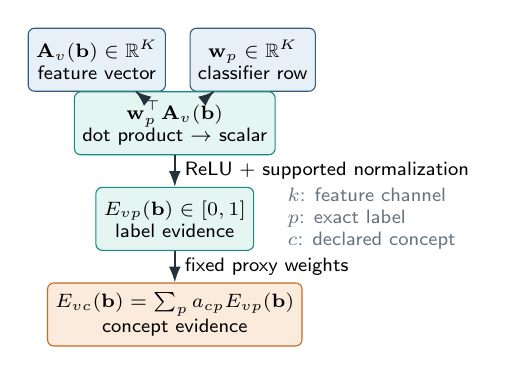
\begin{tikzpicture}[font=\sffamily\scriptsize,>=Latex,
 box/.style={rounded corners=.8mm,draw=ink,align=center,minimum height=8mm,inner sep=1mm},
 arr/.style={->,draw=ink,line width=.6pt}]
\node[box,fill=inputfill,draw=inputblue] (a)
 {$\mathbf A_v(\mathbf b)\in\R^K$\\feature vector};
\node[box,fill=inputfill,draw=inputblue,right=3mm of a] (w)
 {$\mathbf w_p\in\R^K$\\classifier row};
\node[box,fill=evalfill,draw=eval,below=4mm of $(a)!0.5!(w)$] (dot)
 {$\mathbf w_p^\top\mathbf A_v(\mathbf b)$\\dot product $\to$ scalar};
\node[box,fill=evalfill,draw=eval,below=4mm of dot] (ep)
 {$E_{vp}(\mathbf b)\in[0,1]$\\label evidence};
\node[box,fill=propfill,draw=prop,below=4mm of ep] (ec)
 {$E_{vc}(\mathbf b)=\sum_pa_{cp}E_{vp}(\mathbf b)$\\concept evidence};
\draw[arr] (a)--(dot); \draw[arr] (w)--(dot);
\draw[arr] (dot)-- node[right] {ReLU + supported normalization} (ep);
\draw[arr] (ep)-- node[right] {fixed proxy weights} (ec);
\node[align=left,text=muted,anchor=west] at ([xshift=3mm]ep.east)
 {$k$: feature channel\\$p$: exact label\\$c$: declared concept};
\end{tikzpicture}
\caption{Two distinct CAM operations. The first contracts two $K$-vectors into one class score at a bearing. The second combines several scalar label fields into one predeclared concept field. Neither operation produces an object mask.}
\label{fig:camtypes}
\end{figure}

\subsection{Sampling evidence at registered tracks}

For accepted observation $\mathcal O_{tv}$, nearest pixel-centre sampling gives
\begin{equation}
 s_{tvc}=Q_v(\mathbf b_{tv})E_{vc}(\mathbf b_{tv}),
 \quad r_{tv}\le\tau_r,\quad s_{tvc}\ge\tau_o.
 \label{eq:tracksample}
\end{equation}
In Eq.~\ref{eq:tracksample}, $Q_v(\mathbf b_{tv})$ is a Boolean support value
(numerically 0 or 1), $E_{vc}(\mathbf b_{tv})$ is a scalar evidence value, and
their product $s_{tvc}$ is a scalar in $[0,1]$. Nearest pixel-centre sampling
is used because the registered feature names one measurement. The inequalities
are acceptance tests, not additional factors in the product.
Only supported observations enter aggregation. Track evidence uses a geometric mean over its $n_{tc}$ positive evidence-bearing panoramas:
\begin{equation}
 s_{tc}=\exp\!\left[
 \frac{1}{n_{tc}}
 \sum_{v\in\mathcal V^+_{tc}}
 \log\max(s_{tvc},\epsilon)\right].
 \label{eq:geomean}
\end{equation}
This penalizes a track that is strong in one panorama but weak in another. It survives if $s_{tc}\ge\tau_t$. Let $s_{t(1)}$ and $s_{t(2)}$ be its top two concept scores. The ambiguity flag is
\begin{equation}
 a_t=\mathbf 1\!\left[
 s_{t(1)}\ge\tau_t\ \wedge\
 s_{t(1)}-s_{t(2)}<\tau_a\right].
 \label{eq:ambiguity}
\end{equation}
The logarithm and exponential operate on scalars. For two panoramas with
scores $0.8$ and $0.2$, Eq.~\ref{eq:geomean} returns
$\sqrt{0.8\times0.2}=0.4$, whereas an arithmetic mean returns $0.5$. Thus one
weak view has a stronger effect without forcing the score to zero. The output
$a_t\in\{0,1\}$ is a Boolean flag: it becomes one only when the best concept is
acceptable but insufficiently separated from the runner-up.

\subsection{Spatial clustering}

For each concept, candidates are sorted by decreasing $s_{tc}$ and assigned by deterministic complete link. Candidate $t$ can join cluster $K$ only if
\begin{equation}
 \max_{j\in K}\|\mathbf X_t-\mathbf X_j\|_2\le r_c.
 \label{eq:completelink}
\end{equation}
When no metric radius is supplied, $r_c=\alpha B$, where $B$ is the median non-zero camera baseline. Complete link prevents a chain of pairwise-near points from bridging distant instances.

The subtraction $\mathbf X_t-\mathbf X_j$ produces a 3-vector; its Euclidean
norm produces one non-negative distance scalar in the declared world units.
The maximum reduces all pairwise distances from candidate $t$ to cluster $K$
to one worst-case distance. For example, distances
$\{0.2,0.4,1.1\}$ m fail a radius $r_c=1.0$ m even though their mean is below
the threshold. This is precisely the anti-chaining behavior intended by
complete link.

Within cluster $K_i$, let
$\omega_t=s_{tc}/\sum_{j\in K_i}s_{jc}$. Its sparse spatial summary is
\begin{align}
 \bm\mu_i&=\sum_{t\in K_i}\omega_t\mathbf X_t, \label{eq:center}\\
 \bm\Sigma_i&=\sum_{t\in K_i}\omega_t
 (\mathbf X_t-\bm\mu_i)(\mathbf X_t-\bm\mu_i)^\top, \label{eq:cov}\\
 \rho_i&=\max_{t\in K_i}\|\mathbf X_t-\bm\mu_i\|_2. \label{eq:radius}
\end{align}
$\bm\Sigma_i$ and $\rho_i$ describe support spread, not calibrated uncertainty and not full physical extent.
Here $\omega_t$ is a normalized scalar weight with
$\sum_{t\in K_i}\omega_t=1$, $\bm\mu_i\in\R^3$ is a weighted vector average,
and $\rho_i\in\R_{\ge0}$ is one radius scalar. In Eq.~\ref{eq:cov}, the
difference $\Delta_t=\mathbf X_t-\bm\mu_i\in\R^3$ is a column vector and
$\Delta_t\Delta_t^\top\in\R^{3\times3}$ is its outer product. For
$\Delta_t=(d_x,d_y,d_z)^\top$, this matrix has entries
$(\Delta_t\Delta_t^\top)_{ab}=d_a d_b$; diagonal entries measure spread along
the axes and off-diagonal entries measure coupled variation. Summing these
matrices produces $\bm\Sigma_i\in\R^{3\times3}$. Figure~\ref{fig:clustertypes}
shows the three summaries without interpreting them as an object boundary.

\begin{figure}[t]
\centering
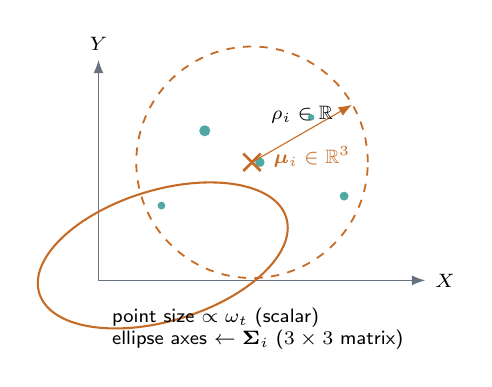
\begin{tikzpicture}[font=\sffamily\scriptsize,>=Latex]
\draw[->,draw=muted] (-2.0,-1.25)--(2.15,-1.25) node[right] {$X$};
\draw[->,draw=muted] (-2.0,-1.25)--(-2.0,1.55) node[above] {$Y$};
\foreach \x/\y/\rad in {-1.20/-.30/1.4,-.65/.65/2.0,.05/.25/1.7,.70/.82/1.2,1.12/-.18/1.6}{
  \fill[eval,opacity=.75] (\x,\y) circle (\rad pt);
}
\draw[prop,line width=.75pt,rotate around={17:(-.05,.25)}]
 (-1.48,-.55) ellipse (1.64 and .83);
\draw[prop,dashed,line width=.65pt] (-.05,.25) circle (1.47);
\draw[prop,line width=1pt] (-.16,.14)--(.06,.36);
\draw[prop,line width=1pt] (-.16,.36)--(.06,.14);
\node[prop,anchor=west] at (.10,.32) {$\bm\mu_i\in\R^3$};
\draw[->,draw=prop] (-.05,.25)--(1.22,.98)
 node[midway,above] {$\rho_i\in\R$};
\node[align=left,anchor=north west] at (-1.95,-1.48)
 {point size $\propto\omega_t$ (scalar)\\ellipse axes $\leftarrow\bm\Sigma_i$ ($3\times3$ matrix)};
\end{tikzpicture}
\caption{Typed spatial summary, drawn in 2-D for readability although the computation is in $\R^3$. Points are accepted sparse estimates, the cross is the weighted mean, the ellipse visualizes second moments, and the dashed circle visualizes the maximum support radius. None is a segmentation mask.}
\label{fig:clustertypes}
\end{figure}
The cluster instantiates the hypothesis fields as
\begin{equation}
 \mathcal T_i=K_i,\qquad
 \mathcal V_i=\bigcup_{t\in K_i}\mathcal V^+_{tc},\qquad
 q_i=\sum_{t\in K_i}\omega_t s_{tc},
 \label{eq:hypothesisfields}
\end{equation}
and $\mathcal S_i=(\kappa_i,\bm\mu_i,\bm\Sigma_i,\rho_i)$, where $\kappa_i$ is inherited from the reconstruction's declared scale contract. The score $q_i$ is used for ranking and is not interpreted as a calibrated probability. The provenance field is
\begin{equation}
 \mathcal P_i=\left(
  \{(\nu_v,\pi_v):v\in\mathcal V_i\},
  \gamma_{\rm geom},\Theta,\chi_i\right),
 \label{eq:provenance}
\end{equation}
where $\gamma_{\rm geom}$ identifies the geometry convention, $\Theta$ is the frozen parameter set, and $\chi_i$ is the reduction and verification trace.

Equation~\ref{eq:hypothesisfields} deliberately mixes three operations with
different output types: assignment preserves the finite set $K_i$ as
$\mathcal T_i$; set union produces the finite panorama-ID set $\mathcal V_i$;
and a weighted sum produces the scalar $q_i$. The enclosing hypothesis in
Eq.~\ref{eq:hypothesis} is therefore a heterogeneous record, not a numeric
array on which vector arithmetic should be applied.

A hypothesis is confirmed only if
\begin{equation}
 |\mathcal T_i|\ge T_{\min},\quad
 |\mathcal V_i|\ge V_{\min}\ge2,\quad
 \frac{\sum_{t\in K_i}a_t}{|K_i|}\le\tau_f.
 \label{eq:confirm}
\end{equation}
If Eq.~\ref{eq:confirm} holds and no hard geometric or vocabulary contradiction is present, $\eta_i=\text{confirmed}$. A surviving cluster with excessive semantic ambiguity or mutually incompatible verification cues has $\eta_i=\text{ambiguous}$; every other surviving candidate has $\eta_i=\text{proposed}$. The reasons are stored in $\chi_i$, so the state is reproducible rather than a visual judgement.

\subsection{Adaptive gnomonic region}

For camera $v$, support point $t$ projects to
\begin{equation}
 \mathbf d_{tv}=\mathbf R_v(\mathbf X_t-\mathbf C_v),\qquad
 \mathbf b'_{tv}=\frac{\mathbf d_{tv}}{\|\mathbf d_{tv}\|_2}.
 \label{eq:project3d}
\end{equation}
The subtraction, rotation, and normalization all act on 3-vectors. Specifically,
$\mathbf X_t-\mathbf C_v\in\R^3$ is a world-frame displacement,
$\mathbf R_v\in\R^{3\times3}$ maps it to a camera-frame displacement
$\mathbf d_{tv}\in\R^3$, and division by the scalar length
$\|\mathbf d_{tv}\|_2$ produces a unit vector
$\mathbf b'_{tv}\in\sphere$. This is a predicted direction and carries no
range after normalization.
The proposed optical axis is the normalized weighted spherical mean
\begin{equation}
 \bar{\mathbf b}_{iv}=\normalize\!\left(
 \sum_{t\in K_i}\omega_t\mathbf b'_{tv}\right).
 \label{eq:meanbearing}
\end{equation}
If the weighted sum is numerically zero, the highest-weight bearing is used.

The weighted sum inside Eq.~\ref{eq:meanbearing} is a 3-vector. Normalization
projects it back to the unit sphere. It is not a mean of ERP pixel coordinates
or longitudes, so directions on opposite sides of the horizontal seam average
correctly. For example, bearings near longitudes $+179^\circ$ and
$-179^\circ$ produce a mean near the seam, not near $0^\circ$.

Let $(\mathbf r,\mathbf u,\mathbf f)$ be the right, up, and forward basis at $\bar{\mathbf b}_{iv}=\mathbf f$. Local offsets are
\begin{equation}
 h_t=\left|\tan^{-1}\frac{\mathbf b'_{tv}\cdot\mathbf r}
 {\mathbf b'_{tv}\cdot\mathbf f}\right|,\quad
 z_t=\left|\tan^{-1}\frac{\mathbf b'_{tv}\cdot\mathbf u}
 {\mathbf b'_{tv}\cdot\mathbf f}\right|.
 \label{eq:offsets}
\end{equation}
With margin $m$ and bounds $\theta_{\min},\theta_{\max}$,
\begin{align}
 \theta_h&=\clip\!\left(2(\max_t h_t+m),
 \theta_{\min},\theta_{\max}\right),\\
 \theta_v&=\clip\!\left(2(\max_t z_t+m),
 \theta_{\min},\theta_{\max}\right).
 \label{eq:fov}
\end{align}
The per-panorama region is therefore the explicit geometric object
\begin{equation}
 R_{iv}=\left(\bar{\mathbf b}_{iv},\mathbf r_{iv},
 \mathbf u_{iv},\theta_{h,iv},\theta_{v,iv}\right),
 \qquad
 \mathcal G_i=\{R_{iv}:v\in\mathcal V_i\}.
 \label{eq:regionobject}
\end{equation}
The local gnomonic ray for tangent coordinates $(\xi,\upsilon)$ is
\begin{equation}
 \mathbf g(\xi,\upsilon)=
 \normalize(\mathbf f+\xi\mathbf r-\upsilon\mathbf u),
 \label{eq:gnomonic}
\end{equation}
with $|\xi|\le\tan(\theta_h/2)$ and
$|\upsilon|\le\tan(\theta_v/2)$.

The basis vectors $\mathbf r,\mathbf u,\mathbf f\in\R^3$ are mutually
orthogonal unit vectors. Each dot product in Eq.~\ref{eq:offsets} returns a
scalar component; their ratio is a dimensionless scalar; and
$\tan^{-1}$ converts that ratio into an angular scalar. In
Eq.~\ref{eq:gnomonic}, $\xi$ and $\upsilon$ are tangent-plane scalars, so the
linear combination is a 3-vector and $\normalize$ returns a unit ray. Thus
$R_{iv}$ is a record containing three vectors and two scalar angles, not a
planar bounding-box array. Figure~\ref{fig:geometry} follows these exact types.

\begin{figure}[t]
\centering
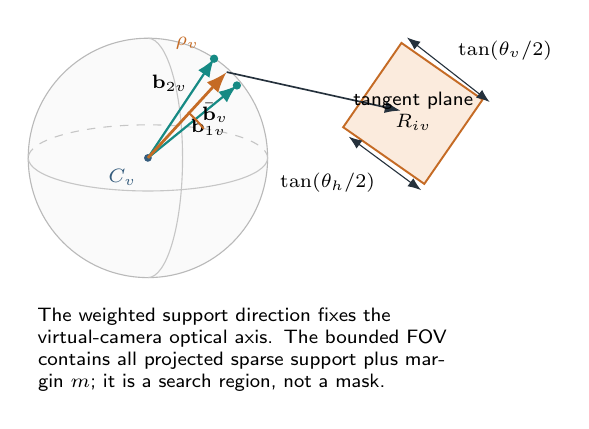
\begin{tikzpicture}[font=\sffamily\scriptsize,>=Latex]
  \coordinate (C) at (0,0);
  \draw[draw=gray!55, fill=gray!4] (C) circle (1.52);
  \draw[draw=gray!45] (-1.52,0) arc[start angle=180,end angle=360,x radius=1.52,y radius=.42];
  \draw[draw=gray!45,dashed] (1.52,0) arc[start angle=0,end angle=180,x radius=1.52,y radius=.42];
  \draw[draw=gray!45] (0,-1.52) arc[start angle=-90,end angle=90,x radius=.44,y radius=1.52];
  \fill[inputblue] (C) circle (1.4pt) node[below left=1pt] {$C_v$};
  \coordinate (b1) at (1.13,.92);
  \coordinate (b2) at (.84,1.26);
  \coordinate (bc) at (1.00,1.09);
  \draw[->,draw=eval,line width=.8pt] (C)--(b1) node[pos=.68,below] {$\mathbf b_{1v}$};
  \draw[->,draw=eval,line width=.8pt] (C)--(b2) node[pos=.75,left] {$\mathbf b_{2v}$};
  \draw[->,draw=prop,line width=1.0pt] (C)--(bc) node[pos=.52,right=1pt] {$\bar{\mathbf b}_v$};
  \fill[eval] (b1) circle (1.5pt);
  \fill[eval] (b2) circle (1.5pt);
  \draw[draw=prop,line width=.75pt] (.51,.58) arc[start angle=49,end angle=38,radius=1.50];
  \node[text=prop] at (.50,1.46) {$\rho_v$};
  \coordinate (P0) at (2.48,.39);
  \coordinate (P1) at (3.22,1.46);
  \coordinate (P2) at (4.25,.74);
  \coordinate (P3) at (3.51,-.33);
  \draw[fill=propfill,draw=prop,line width=.7pt] (P0)--(P1)--(P2)--(P3)--cycle;
  \draw[->,draw=ink,line width=.6pt] (bc)--(3.21,.60);
  \node[align=center,text width=20mm] at (3.37,.59) {tangent plane\\$R_{iv}$};
  \draw[<->,draw=ink] (2.55,.27)--(3.47,-.41) node[midway,below left] {$\tan(\theta_h/2)$};
  \draw[<->,draw=ink] (4.34,.71)--(3.29,1.53) node[midway,above right] {$\tan(\theta_v/2)$};
  \node[anchor=north west,align=left,text width=52mm] at (-1.52,-1.78) {The weighted support direction fixes the virtual-camera optical axis. The bounded FOV contains all projected sparse support plus margin $m$; it is a search region, not a mask.};
\end{tikzpicture}
\caption{Per-panorama region construction. Reprojected support bearings $\mathbf b'_{tv}\in\sphere$ determine the unit-vector mean $\bar{\mathbf b}_{iv}\in\sphere$. That vector is the forward axis $\mathbf f$ of an orthonormal $3\times3$ local frame; scalar half-angle tangents determine the plane extent. The resulting footprint is a typed search-region record, not an object mask.}
\label{fig:geometry}
\end{figure}

The intended optimization target is not the exact object peak. It is the smallest stable region expected to retain most relevant evidence:
\begin{equation}
 R^*=\arg\max_R
 \left[
 C_{\rm obj}(R)-\lambda\Omega(R)-\mu C_{\rm bg}(R)
 \right],
 \label{eq:regionutility}
\end{equation}
where $C_{\rm obj}$ is object/evidence coverage, $\Omega$ is solid angle, and $C_{\rm bg}$ is contamination. Equation~\ref{eq:regionutility} will be evaluated through measurable surrogates rather than optimized using test annotations.

Every term inside the brackets is scalar. The non-negative weights
$\lambda$ and $\mu$ convert angular cost and contamination to the same ranking
scale as coverage. The $\arg\max$ operator returns the region object $R^*$ that
attains the largest utility; it returns neither the maximum scalar value nor a
pixel mask.

\subsection{Detector-style spherical FOV anchors}

The sparse-support region above is a search region. An object extent is
inferred independently in each panorama from a local CAM component. Let
$R^0_{kv}$ be the base region for local component $k$ in view $v$, with
horizontal and vertical fields of view $(\theta^0_h,\theta^0_v)$. A finite
anchor family is generated from scale $s\in\mathcal S$ and aspect ratio
$a\in\mathcal A$:
\begin{align}
 \theta_h(s,a)&=\clip(s\sqrt a\,\theta^0_h,
 \theta_{\min},\theta_{\max}),\\
 \theta_v(s,a)&=\clip(s/\sqrt a\,\theta^0_v,
 \theta_{\min},\theta_{\max}).
 \label{eq:anchorfamily}
\end{align}
All variants retain the same spherical centre and an explicit proposal-family
identifier $f_{kv}$ tied to the original local component. The identifier is
not a semantic hypothesis ID: one upstream hypothesis may contain several
disconnected components or physical instances.

Within one view and concept, solid-angle IoU provides spherical NMS. Cross-view
anchors use hard vocabulary and geometric gates followed by alternative
identity cues. If $g_{ij}$ is geometric compatibility and
$c\in\mathcal C_{ij}$ indexes the available transfer, track, and appearance
cues, the anchor affinity is
\begin{equation}
 A^{\rm anchor}_{ij}=g_{ij}
 \left[1-\prod_{c\in\mathcal C_{ij}}(1-s_{ijc})^{w_c}\right].
 \label{eq:anchoraffinity}
\end{equation}
An unavailable cue is absent from $\mathcal C_{ij}$; an observed zero remains
zero support. Complete-link clustering admits a new view only when it exceeds
the threshold against every current member, preventing an $A$--$B$--$C$
single-link bridge. At most one anchor from each panorama may enter a cluster.

For a selected cluster $D$ and target view $v$, let $M_v$ be its local anchor
mask and $\Pi_{u\rightarrow v}(M_u)$ an available registered transfer. The
transient consensus field is
\begin{equation}
 Z_v(x)=\frac{M_v(x)+
 \sum_{u\in D\setminus v}A^{\rm anchor}_{uv}
 \Pi_{u\rightarrow v}(M_u)(x)}
 {1+\sum_{u\in D\setminus v}A^{\rm anchor}_{uv}}.
 \label{eq:anchorconsensus}
\end{equation}
After thresholding $Z_v$, the method refits the smallest bounded gnomonic FOV
that contains the configured solid-angle coverage plus margin. Raster masks
are then released. Cluster-level NMS suppresses an alternative only when its
complete set of proposal-family IDs matches a stronger cluster and its
view-wise consensus regions meet the overlap threshold. Accumulated upstream
lineage alone never suppresses a candidate.

\subsection{Pairwise consistency}

For region track sets $T_A$ and $T_B$, implemented identity evidence is
\begin{align}
 J_T(A,B)&=\frac{|T_A\cap T_B|}{|T_A\cup T_B|}, \label{eq:jaccard}\\
 C_T(A,B)&=\frac{|T_A\cap T_B|}
 {\min(|T_A|,|T_B|)}. \label{eq:trackcoverage}
\end{align}
$T_A$ and $T_B$ are finite sets of integer track IDs. Intersection and union
therefore produce sets, while vertical bars produce integer cardinalities; the
ratios are scalar scores in $[0,1]$. If
$T_A=\{1,2,3\}$ and $T_B=\{2,3,4,5\}$, then
$J_T=2/5=0.4$ and $C_T=2/3\approx0.67$. Jaccard penalizes all unmatched
tracks; smaller-view coverage asks whether the smaller region is mostly
contained in the larger one.
For shared tracks $\mathcal S_{AB}$ and reprojection residual
$e_{tv}$, define robust geometric agreement
\begin{equation}
 S_{\rm reproj}(A,B)=
 \exp\!\left[
 -\frac{\operatorname{median}_{t\in\mathcal S_{AB}}
 (e_{tA}+e_{tB})}{2\sigma_r}\right].
 \label{eq:reproj}
\end{equation}

An optional caller-owned face encoder gives vectors
$\mathbf e_A,\mathbf e_B$ under one frozen preprocessing path:
\begin{equation}
 S_{\rm app}(A,B)=
 \frac{\mathbf e_A^\top\mathbf e_B}
 {\|\mathbf e_A\|_2\|\mathbf e_B\|_2}.
 \label{eq:cosine}
\end{equation}
Appearance complements but never replaces registered correspondence.

In Eq.~\ref{eq:reproj}, every $e_{tv}$ and $\sigma_r$ is an angular scalar in
the same unit; the median, division, negation, and exponential yield one score
in $(0,1]$. In Eq.~\ref{eq:cosine}, both embeddings are vectors in the same
space $\R^D$. The numerator is a scalar dot product and each denominator term
is a scalar length, so $S_{\rm app}\in[-1,1]$. Comparing embeddings of
different dimension or preprocessing provenance is undefined and must fail.

\subsection{Symmetric regional transfer}

Regions $R_A$ and $R_B$ must be inferred independently. Pixels or support from $R_A$ are transferred through registered radial depth or 3-D points into $B$, yielding $\Pi_{A\rightarrow B}(R_A)$. Solid-angle-weighted overlap is
\begin{equation}
 \IoU_{A\rightarrow B}=
 \frac{\sum_{x\in\Omega_B}w_x
 \mathbf1[x\in\Pi_{A\rightarrow B}(R_A)\cap R_B]}
 {\sum_{x\in\Omega_B}w_x
 \mathbf1[x\in\Pi_{A\rightarrow B}(R_A)\cup R_B]},
 \quad w_x=\cos\varphi_x.
 \label{eq:transferiou}
\end{equation}
Here $x$ indexes discrete pixels in panorama $B$, $w_x$ is a non-negative
scalar approximating that pixel's solid angle, and $\mathbf1[\cdot]$ is a
Boolean indicator converted to 0 or 1. The numerator sums the solid angle of
the transferred intersection; the denominator sums the solid angle of the
union. Thus the quotient is a scalar in $[0,1]$ and is not biased by the large
ERP pixel count near the poles. $\Pi_{A\rightarrow B}$ is an operator from one
region record plus registered geometry to a set of target pixels; it is not a
matrix multiplication.
The symmetric regional score is
\begin{equation}
 S_{\rm IoU}(A,B)=\frac12
 \left(\IoU_{A\rightarrow B}+
 \IoU_{B\rightarrow A}\right).
 \label{eq:symiou}
\end{equation}
Projecting one common 3-D region into both views and measuring agreement would be tautological and is excluded.

The average in Eq.~\ref{eq:symiou} combines two scalar measurements computed
on different target lattices. Its symmetry is operational: swapping $A$ and
$B$ leaves the final score unchanged, even though the two directional IoUs can
differ because support and discretization differ.

\subsection{Affinity, fusion, and spherical Soft-NMS}

For hypotheses $i,j$, define factors in $[0,1]$: semantic compatibility $S_{\rm sem}$, 3-D compatibility $S_{\rm geo}$, track consistency $S_{\rm trk}$, transfer $S_{\rm IoU}$, and shifted appearance
$S_{\rm app}^+=(1+S_{\rm app})/2$. The affinity is
\begin{equation}
 A_{ij}=S_{\rm sem}^{\alpha}
 S_{\rm geo}^{\beta}
 S_{\rm trk}^{\gamma}
 S_{\rm IoU}^{\delta}
 (S_{\rm app}^{+})^{\epsilon}.
 \label{eq:affinity}
\end{equation}
A missing optional cue removes its factor rather than forcing zero. Hard gates first reject incompatible vocabularies, contradictory geometry, or depth-separated support. Edges above $\tau_A$ define possible duplicate components.

Every factor and exponent in Eq.~\ref{eq:affinity} is scalar. Taking logs makes
the product especially easy to audit:
$\log A_{ij}=\alpha\log S_{\rm sem}+\beta\log S_{\rm geo}+cdots$.
The exponents therefore control relative influence without changing data type.
For example, with two equally weighted available cues $0.8$ and $0.5$, the
affinity is $0.4$; an unavailable optional cue is omitted, whereas an observed
cue equal to zero is decisive evidence and makes the product zero.

Within compatible component $D$, fusion occurs in $\R^3$:
\begin{equation}
 \bm\mu_D=
 \frac{\sum_{i\in D}\gamma_i\bm\mu_i}
 {\sum_{i\in D}\gamma_i},
 \qquad
 \gamma_i=q_i g_i u_i,
 \label{eq:fusion}
\end{equation}
where $q_i$ is semantic confidence, $g_i$ geometric quality, and $u_i$ an independent-view factor. Longitude is never averaged directly.

$\gamma_i=q_i g_i u_i$ is a scalar fusion weight and each
$\bm\mu_i\in\R^3$, so both the numerator and the result in
Eq.~\ref{eq:fusion} are 3-vectors. This is a weighted Euclidean average of
compatible 3-D supports. Direction-only hypotheses require spherical vector
averaging instead and cannot be silently inserted into this metric equation.

For an unfused alternative $j$ against selected hypothesis $i$, spherical Soft-NMS gives
\begin{equation}
 q'_j=q_j\exp\!\left(-\frac{O_{ij}^2}{\sigma}\right),
 \label{eq:softnms}
\end{equation}
where $O_{ij}$ combines transferred spherical overlap and 3-D support overlap. Incompatible concepts and depth-separated instances remain concurrent.

Equation~\ref{eq:softnms} maps the original scalar score $q_j$ to another
scalar $q'_j$. It does not modify the hypothesis region or spatial support.
When $O_{ij}=0$, the exponential is one and the score is unchanged; increasing
overlap continuously reduces the score, with $\sigma>0$ controlling the decay.

\begin{figure*}[t]
\centering
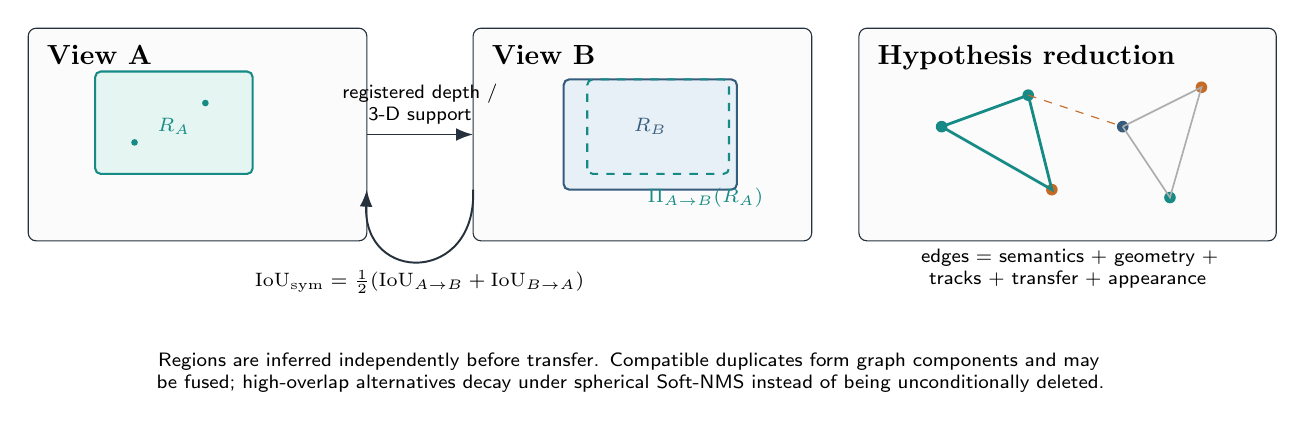
\begin{tikzpicture}[
  font=\sffamily\scriptsize,
  >=Latex,
  view/.style={rounded corners=1mm, draw=ink, fill=gray!3, minimum width=43mm, minimum height=27mm},
  hyp/.style={rounded corners=.7mm, line width=.75pt},
  arrow/.style={->,line width=.7pt,draw=ink}
]
\node[view] (A) at (0,0) {};
\node[anchor=north west,font=\bfseries] at ([xshift=1.2mm,yshift=-1mm]A.north west) {View A};
\draw[hyp,draw=eval,fill=evalfill] ([xshift=-13mm,yshift=-5mm]A.center) rectangle ++(20mm,13mm);
\node[text=eval] at ([xshift=-3mm,yshift=1mm]A.center) {$R_A$};
\fill[eval] ([xshift=-8mm,yshift=-1mm]A.center) circle (1.2pt);
\fill[eval] ([xshift=1mm,yshift=4mm]A.center) circle (1.2pt);
\node[view] (B) at (5.65,0) {};
\node[anchor=north west,font=\bfseries] at ([xshift=1.2mm,yshift=-1mm]B.north west) {View B};
\draw[hyp,draw=inputblue,fill=inputfill] ([xshift=-10mm,yshift=-7mm]B.center) rectangle ++(22mm,14mm);
\node[text=inputblue] at ([xshift=1mm,yshift=1mm]B.center) {$R_B$};
\draw[hyp,draw=eval,dashed] ([xshift=-7mm,yshift=-5mm]B.center) rectangle ++(18mm,12mm);
\node[text=eval] at ([xshift=8mm,yshift=-8mm]B.center) {$\Pi_{A\rightarrow B}(R_A)$};
\draw[arrow] ([xshift=21.5mm]A.center) -- node[above,align=center] {registered depth /\\3-D support} ([xshift=-21.5mm]B.center);
\draw[arrow] ([xshift=-21.5mm,yshift=-7mm]B.center) .. controls (3.55,-1.9) and (2.10,-1.9) .. ([xshift=21.5mm,yshift=-7mm]A.center);
\node[align=center] at (2.82,-1.87) {$\mathrm{IoU}_{\rm sym}=\frac12(\mathrm{IoU}_{A\to B}+\mathrm{IoU}_{B\to A})$};
\node[rounded corners=1mm,draw=ink,fill=gray!3,minimum width=53mm,minimum height=27mm] (G) at (11.05,0) {};
\node[anchor=north west,font=\bfseries] at ([xshift=1.2mm,yshift=-1mm]G.north west) {Hypothesis reduction};
\foreach \x/\y/\c/\name in {-16/1/eval/h1,-5/5/eval/h2,7/1/inputblue/h3,17/6/prop/h4,-2/-7/prop/h5,13/-8/eval/h6}{
  \fill[\c] ([xshift=\x mm,yshift=\y mm]G.center) circle (2.1pt) coordinate (\name);
}
\draw[draw=eval,line width=1pt] (h1)--(h2)--(h5)--(h1);
\draw[draw=gray!65,line width=.6pt] (h3)--(h4)--(h6)--(h3);
\draw[draw=prop,dashed] (h2)--(h3);
\node[align=center,text width=44mm] at ([yshift=-17mm]G.center) {edges = semantics + geometry + tracks + transfer + appearance};
\node[align=center,text width=150mm,anchor=north west] at (-2.15,-2.65) {Regions are inferred independently before transfer. Compatible duplicates form graph components and may be fused; high-overlap alternatives decay under spherical Soft-NMS instead of being unconditionally deleted.};
\end{tikzpicture}
\caption{Implemented regional transfer and detector-style reduction. Transfer is measured in both directions between independently inferred regions. The reduction graph combines semantic, spherical, track, geometric, and optional appearance evidence; the evaluation programme tests its accuracy and failure modes.}
\label{fig:transfer}
\end{figure*}

\subsection{Optional boundary refinement}

Segmentation is downstream, not constitutive. A confirmed region may prompt SAM or another mask generator if an operation needs a boundary. Multiple masks are retained as alternatives. A mask is associated back to the same hypothesis only if it satisfies support, stability, overlap, and cross-face continuity criteria. Failure to segment does not erase an otherwise coherent spatial association.

\section{Experimental Design}

\subsection{Research questions}

The study will answer six questions:
\begin{enumerate}
 \item \textbf{RQ1 -- Regional utility:} Does the mean-direction gnomonic region retain more class/object evidence than expected from its solid-angle cost?
 \item \textbf{RQ2 -- Multiview association:} Are independently generated regions for the same physical hypothesis consistent under registered transfer, tracks, local features, and embeddings?
 \item \textbf{RQ3 -- Spherical inference:} Does direct-spherical inference match or improve regional utility and cost relative to naive ERP and multiface inference?
 \item \textbf{RQ4 -- Semantic source:} How do architecture capacity, closed versus open vocabulary, and industrial specialization affect the hypotheses?
 \item \textbf{RQ5 -- Reduction:} Can affinity fusion and spherical Soft-NMS reduce fragmentation without losing distinct nearby instances?
 \item \textbf{RQ6 -- Efficiency and robustness:} What time, memory, and accuracy trade-offs arise under ERP resolution, geometric noise, support loss, seams, and poles?
\end{enumerate}

\subsection{Datasets and evidence strata}

Evaluation will use three disjoint strata:
\begin{itemize}
 \item \textbf{Analytic/synthetic:} known spherical regions crossing the ERP seam, approaching poles, overlapping in angle but separated in depth, and partially outside support.
 \item \textbf{Stanford2D3D:} registered indoor panoramas with semantic labels, used only under its data agreement.
 \item \textbf{Matterport3D:} registered indoor scenes with object/region annotations where licensing permits the required measurements.
\end{itemize}
Dataset-specific adapters remain outside the generic API. Scene groups, rather than individual windows, are the unit of training, validation, and test separation and statistical resampling.

\subsection{Semantic models and vocabularies}

The frozen model matrix is designed to separate architecture strength from vocabulary:
\begin{table}[H]
\centering
\caption{Planned semantic evidence factors. Every checkpoint, preprocessing recipe, label list, and hash will be frozen before evaluation.}
\label{tab:models}
\begin{tabular}{@{}p{18mm}p{21mm}p{28mm}@{}}
\toprule
Family & Models & Purpose\\
\midrule
ImageNet CNN & VGG-16, ResNet-18, ResNet-152, EfficientNet-B3, EfficientNet-B7 & classic baseline, current reference, deeper residual, intermediate and high-capacity efficient models\\
Places365 CNN & ResNet-18 & fixed scene vocabulary and context evidence\\
OpenCLIP & RN50 & open-vocabulary spatial similarity, reported separately from classifier CAM\\
Industrial CNN & frozen private ResNet-18 & domain-specialized comparison, never a public checkpoint\\
\bottomrule
\end{tabular}
\end{table}

ImageNet industrial proxies are fixed in advance for concepts such as piping, cylindrical vessels, access structures, panels, and metallic framework. Exact proxy labels and weights are reported with every result. Places365 tests whether scene context improves proposal ranking rather than pretending to be an object label. OpenCLIP RN50 is evaluated as a separate open-vocabulary evidence source because its spatial similarity map is not identical to a linear classification CAM.

\subsection{Inference baselines}

Each eligible closed-set CNN is evaluated under:
\begin{enumerate}
 \item \textbf{Direct sphere:} ported weights with spherical sampling on the full ERP.
 \item \textbf{Naive ERP:} conventional planar convolutions applied directly to ERP, exposing latitude distortion.
 \item \textbf{Multiface:} the unchanged planar model on overlapping gnomonic faces, with spherical backprojection and overlap fusion.
\end{enumerate}
The multiface baseline reports face count, FOV, overlap, aggregation, and actual peak memory. Faces are streamed so storage policy does not unfairly inflate memory. The semantic output is compared at matched angular sampling density whenever feasible.

\subsection{Proposal baselines and ablations}

The following proposal variants isolate each contribution:
\begin{itemize}
 \item CAM maximum with fixed FOV;
 \item spherical CAM centroid with fixed FOV;
 \item registered-track mean direction with fixed FOV;
 \item adaptive FOV from sparse support (full candidate core);
 \item geometry-only proposals without semantic weighting;
 \item semantics-only bearing proposals without tracks;
 \item arithmetic versus geometric cross-view score aggregation;
 \item single proxy versus fixed multi-proxy concept;
 \item complete-link versus single-link and centroid clustering;
 \item tracks only, tracks plus embedding, tracks plus transfer IoU, and full affinity;
 \item hard NMS, Soft-NMS, weighted fusion, and fusion plus Soft-NMS; and
 \item optional SAM refinement after association versus no boundary refinement.
\end{itemize}

\subsection{Leave-one-view-out protocol}

For $V\ge3$, fold $h$ removes evidence record $\mathcal D_h$ from registered panorama $h$ while leaving that panorama's camera geometry and tracks fixed. Hypotheses are generated from
$\mathcal V\setminus\{h\}$ and projected into $h$. The held-out CAM or annotation is opened only for scoring. This is the primary semantic-transfer protocol.

A stricter secondary protocol rebuilds registration without the held-out panorama and then registers the panorama as a query. Results from fixed geometry and rebuilt geometry are never pooled. Thresholds, proxy weights, model resolution, cluster radius, and FOV policy are frozen on development scenes.

\section{Evaluation Measures}

\subsection{Regional coverage and angular cost}

For held-out concept field $E_{hc}$, support $Q_h$, region $R$, and
$w_x=\cos\varphi_x$, semantic-mass recall is
\begin{equation}
 R_{\rm mass}=
 \frac{\sum_x w_x Q_h(x)E_{hc}(x)\mathbf1[x\in R]}
 {\sum_x w_x Q_h(x)E_{hc}(x)}.
 \label{eq:mass}
\end{equation}
The fraction of observed sphere consumed is
\begin{equation}
 F_\Omega=
 \frac{\sum_x w_xQ_h(x)\mathbf1[x\in R]}
 {\sum_x w_xQ_h(x)}.
 \label{eq:spherefraction}
\end{equation}
Mean-score enrichment is
\begin{equation}
 G=
 \frac{
 (\sum_{x\in R}w_xQE)/(\sum_{x\in R}w_xQ)}
 {(\sum_xw_xQE)/(\sum_xw_xQ)}.
 \label{eq:enrichment}
\end{equation}
These equations reduce arrays to scalars. For every pixel index $x$,
$w_x\in\R_{\ge0}$ is an area weight, $Q_h(x)\in\{0,1\}$ is support,
$E_{hc}(x)\in[0,1]$ is evidence, and $\mathbf1[x\in R]\in\{0,1\}$ is region
membership. Their product is one non-negative scalar contribution. Summing over
pixels produces scalar masses or areas; dividing matching quantities produces
dimensionless ratios. In Eq.~\ref{eq:mass}, the numerator is evidence mass
inside $R$ and the denominator is all supported evidence mass. In
Eq.~\ref{eq:spherefraction}, both terms are solid-angle surrogates. Equation
\ref{eq:enrichment} divides the mean evidence inside $R$ by the global mean.
We report the coverage-cost curve
$R_{\rm mass}(F_\Omega)$, area under that curve, and the smallest region satisfying target coverage $\kappa$:
\begin{equation}
 F_\Omega^{@\kappa}=
 \min_R\{F_\Omega(R):R_{\rm mass}(R)\ge\kappa\}.
 \label{eq:coveragecost}
\end{equation}
The braces in Eq.~\ref{eq:coveragecost} define a set of admissible regions, not
a numeric vector. The constraint retains regions whose scalar mass recall is at
least the scalar target $\kappa$; $\min_R$ returns the smallest scalar angular
fraction among them. Figure~\ref{fig:metrictypes} provides a visual reading of
the factors in each pixel contribution.

\begin{figure}[t]
\centering
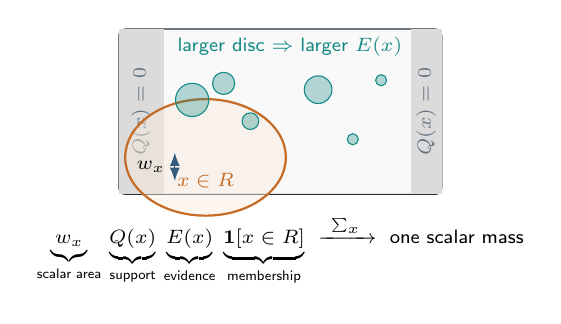
\begin{tikzpicture}[font=\sffamily\scriptsize,>=Latex]
\draw[rounded corners=.8mm,fill=gray!5,draw=ink] (-2.05,-1.05) rectangle (2.05,1.05);
\fill[gray!28] (-2.05,-1.05) rectangle (-1.48,1.05);
\fill[gray!28] (1.66,-1.05) rectangle (2.05,1.05);
\node[rotate=90,text=muted] at (-1.77,0) {$Q(x)=0$};
\node[rotate=90,text=muted] at (1.85,0) {$Q(x)=0$};
\draw[prop,line width=.8pt,fill=propfill,fill opacity=.45]
 (-.95,-.58) ellipse (1.02 and .74);
\node[prop] at (-.95,-.88) {$x\in R$};
\foreach \x/\y/\r in {-1.12/.15/6,-.72/.36/4,-.38/-.12/3,.48/.28/5,.92/-.35/2,1.28/.40/2}{
 \fill[eval,opacity=.32] (\x,\y) circle (\r pt);
 \draw[eval] (\x,\y) circle (\r pt);
}
\node[anchor=south west,text=eval] at (-1.43,.58) {larger disc $\Rightarrow$ larger $E(x)$};
\draw[<->,draw=inputblue] (-1.34,-.88)--(-1.34,-.52)
 node[midway,left] {$w_x$};
\node[align=center,anchor=north] at (0,-1.20)
 {$\underbrace{w_x}_{\text{scalar area}}\,
  \underbrace{Q(x)}_{\text{support}}\,
  \underbrace{E(x)}_{\text{evidence}}\,
  \underbrace{\mathbf1[x\in R]}_{\text{membership}}
  \ \xrightarrow{\ \sum_x\ }\ \text{one scalar mass}$};
\end{tikzpicture}
\caption{Typed reading of the regional metrics on an ERP lattice. Each pixel contributes a product of four scalars. Gray columns are unsupported and contribute zero; colored discs illustrate evidence magnitude; the orange ellipse is region membership. Latitude-dependent $w_x$ corrects the unequal solid angle of ERP pixels.}
\label{fig:metrictypes}
\end{figure}
Where object annotations exist, $E$ is replaced by the instance mask to obtain annotation recall, precision, and solid-angle IoU. Metrics are reported for all proposals and for confirmed proposals, never only successful centre hits.

\subsection{Association quality}

Association is measured by:
\begin{itemize}
 \item symmetric transfer IoU (Eq.~\ref{eq:symiou});
 \item shared-track count, track Jaccard, and smaller-view coverage;
 \item median angular reprojection residual;
 \item local keypoint inlier ratio after region extraction;
 \item optional frozen-encoder cosine similarity;
 \item hypothesis repeatability across view subsets; and
 \item identity precision/recall when persistent instance identifiers exist.
\end{itemize}
Point percentile at the mean direction is retained only as a secondary diagnostic; the main target is region coverage and cross-view consistency.

\subsection{Reduction quality}

Before and after reduction, we measure
\begin{align}
 D_{\rm dup}&=1-\frac{N_{\rm matched\ identities}}{N_{\rm proposals}}, \label{eq:duprate}\\
 F_{\rm frag}&=\frac{1}{N_{\rm objects}}\sum_o N_{\rm hypotheses}(o), \label{eq:frag}\\
 R_{\rm kept}&=\frac{N_{\rm objects\ retained}}{N_{\rm objects\ before}}, \label{eq:kept}
\end{align}
plus average proposals per steradian, recall at fixed proposal budget, precision-recall, and calibration of hypothesis state. Nearby same-class instances form a dedicated preservation test: reduction fails if it improves duplicate rate by merging physically distinct objects.

All $N_{\cdot}$ terms in Eqs.~\ref{eq:duprate}--\ref{eq:kept} are integer
counts. The sums range over object IDs, and the divisions produce scalar rates.
$F_{\rm frag}=1$ means one hypothesis per object on average; values above one
indicate fragmentation. The retained-recall ratio is only meaningful when its
denominator is non-zero, a case handled explicitly rather than by adding an
arbitrary epsilon.

\subsection{Efficiency}

For every inference route we record:
\begin{itemize}
 \item wall time per panorama and per megapixel;
 \item median and P95 after warm-up;
 \item peak resident and accelerator memory;
 \item number of semantic forward passes and projected faces;
 \item total processed pixels, including overlap;
 \item temporary bytes written and lifetime of each face; and
 \item downstream region-verification time.
\end{itemize}
The main efficiency score is useful regional recall per unit work:
\begin{equation}
 \mathcal E_\kappa=
 \frac{\operatorname{Recall}@\kappa}
 {t_{\rm total}\,M_{\rm peak}},
 \label{eq:efficiency}
\end{equation}
reported alongside raw quantities so the compound score cannot hide a bottleneck.

$\operatorname{Recall}@\kappa$ is dimensionless, $t_{\rm total}$ is a scalar
time, and $M_{\rm peak}$ is a scalar memory amount. Consequently
$\mathcal E_\kappa$ has units of inverse time-memory. It is suitable only for
ranking runs measured under the same hardware and measurement protocol; it is
not an intrinsic property of the model.

\subsection{Robustness and geometric correctness}

Analytic tests cover:
\begin{itemize}
 \item ERP seam equivalence under longitude wrap;
 \item north/south pole limits and undefined exact-pole longitude;
 \item partial support and invalid numeric data;
 \item non-square ERP and gnomonic resolutions;
 \item nearest sampling for labels/masks and differentiable bilinear sampling for floating evidence;
 \item face-to-sphere-to-face mask IoU;
 \item pose perturbation, radial-depth noise, track dropout, and outlier tracks;
 \item decreasing view overlap and two-view degeneracy;
 \item FOV saturation at $\theta_{\max}$;
 \item proxy removal, weight perturbation, and competing concepts; and
 \item deterministic output under input reordering.
\end{itemize}

For perturbation magnitude $\delta$, performance degradation is
\begin{equation}
 \Delta m(\delta)=m(0)-m(\delta),
 \label{eq:robustness}
\end{equation}
and a robustness curve is reported rather than one arbitrary noise level.

Both $m(0)$ and $m(\delta)$ are scalar values of the same metric, so their
difference is dimensionally valid. The perturbation $\delta$ must retain its
own unit---degrees for rotation noise, metres for metric translation noise, or
a dimensionless fraction for dropout---and curves with different units are not
pooled.

\section{Experimental Matrix and Acceptance Criteria}

\begin{table*}[t]
\centering
\caption{Pre-specified experiment matrix. Each row produces both aggregate metrics and auditable per-hypothesis records.}
\label{tab:matrix}
\begin{tabular}{@{}p{24mm}p{39mm}p{41mm}p{47mm}@{}}
\toprule
Experiment & Controlled factors & Primary measures & Required interpretation\\
\midrule
Geometry oracle & seam, pole, support, FOV, depth, pose & round-trip IoU, angular error, support correctness & mathematical validity before learned-model evaluation\\
Inference route & direct sphere, naive ERP, streamed multiface & CAM equivalence, regional utility, time, peak memory & quality-efficiency trade-off without hidden face storage\\
Resolution/stride & ERP scale, native feature stride, optional dilation & CAM lattice density, $R_{\rm mass}$--$F_\Omega$ curve & verify FCN density and locate saturation\\
Backbone & VGG-16, ResNet-18/152, EfficientNet-B3/B7 & regional utility, repeatability, compute & architecture effect under fixed vocabulary\\
Vocabulary & ImageNet proxies, Places365, OpenCLIP, industrial model & concept coverage, abstention, association & closed/open/domain evidence reported separately\\
Region rule & peak, centroid, fixed FOV, adaptive FOV & annotation/CAM coverage, angular cost & determine whether mean-direction regions outperform points\\
Association & semantics, tracks, transfer, embedding combinations & transfer IoU, identity precision/recall, calibration & quantify contribution of each independent cue\\
Reduction & hard NMS, Soft-NMS, fusion, combined & duplicate rate, fragmentation, retained recall & remove duplicates without merging distinct objects\\
Boundary refinement & none versus prompted masks & boundary IoU, added cost, association stability & segmentation remains optional and downstream\\
\bottomrule
\end{tabular}
\end{table*}

The methodology is considered supported only if all of the following hold on held-out scenes:
\begin{enumerate}
 \item adaptive regions improve the coverage-cost curve over peak and fixed-FOV baselines;
 \item direct-spherical inference preserves matched-density multiface regional utility while reducing work or peak memory;
 \item multiview cues improve association over proposals using semantics alone;
 \item reduction lowers duplicates/fragmentation without a material loss of distinct-object recall;
 \item improvements persist across scene-blocked confidence intervals rather than one selected panorama; and
 \item all seam, pole, support, and deterministic geometry gates pass.
\end{enumerate}
If these conditions do not hold, the method remains a directional proposal heuristic. A visually convincing overlay is not accepted as evidence.

\section{Statistical and Reproducibility Protocol}

All model identifiers, label vocabularies, hashes, proxy mappings, resolutions, thresholds, and preprocessing recipes are frozen before test evaluation. Hyperparameters are selected on development scenes and used unchanged on held-out Stanford2D3D and Matterport3D scenes.

The primary sampling unit is the scene. We report medians, P95 where appropriate, and 95\% scene-blocked bootstrap intervals. Paired variants use identical scenes, views, tracks, and random seeds. For metric difference $d_s$ on scene $s$, the reported effect is
\begin{equation}
 \bar d=\frac{1}{S}\sum_{s=1}^{S}d_s,
 \label{eq:effect}
\end{equation}
with a paired scene-bootstrap interval. Multiple ablations are interpreted by effect size and interval, not only a null-hypothesis $p$-value.

Here $S$ is an integer number of scenes, each $d_s\in\R$ is one paired scalar
difference computed within scene $s$, and $\bar d\in\R$ is their arithmetic
mean. Resampling draws scene IDs and carries all views from a selected scene
together; treating panoramas from one scene as independent samples would
understate uncertainty.

Every hypothesis record stores model hash, source IDs, exact proxies, track IDs, panorama IDs, camera geometry, thresholds, region specification, state reasons, optional embedding source, and reduction lineage. Public and private cohorts are never pooled into one headline number. Source-checkout, installed-wheel, and external-service evidence are labelled separately.

\section{Threats to Validity}

CAM is discriminative rather than exhaustive, so even a correct hypothesis may cover only an object part. Proxy labels may react to shape or texture without representing the intended industrial concept. Reconstruction points are biased toward textured surfaces and may undersample pipes, homogeneous vessels, or reflective metal. Pose/depth errors can mimic association failure. Open-vocabulary similarity is not calibrated to closed-set CAM and must be analysed separately. Stanford2D3D and Matterport3D do not reproduce all industrial conditions and cannot alone establish generalization.

The design mitigates these threats by separating semantic, geometric, transfer, and appearance evidence; retaining abstention; reporting all proposals rather than selected examples; evaluating coverage and solid angle jointly; and freezing the test protocol. It does not remove the need for broader independent data.

\section{Conclusion}

This paper specifies a training-free method that converts direct-spherical classifier evidence into multiview spatial region hypotheses. The central abstraction is an adaptive gnomonic region around a weighted mean direction, supported by registered tracks and projected consistently into every view. CAM supplies semantics, geometry supplies identity, local faces supply optional verification, and a detector-inspired reducer controls duplicate hypotheses. The proposed evaluation is designed to determine whether these regions retain useful object evidence at lower computational cost than multiface processing and whether cross-view agreement is sufficient for reliable association. Until those experiments are completed, the contribution is a falsifiable methodology and reproducible test plan, not a performance claim.

\section*{Code and Data Plan}

The reusable interfaces belong to the Experimental object localization namespace. Dataset adapters, checkpoints, and training assets remain outside the distributable library. Temporary gnomonic faces are deleted after local evaluation; compact regions, masks where authorized, metrics, and provenance are retained. Public release of any qualitative panel requires a separate license check.

\balance
\begin{thebibliography}{99}

\bibitem[Bodla et~al.(2017)Bodla, Singh, Chellappa, and Davis]{bodla2017softnms}
Bodla, N., Singh, B., Chellappa, R., Davis, L.~S., 2017.
Soft-NMS -- Improving Object Detection With One Line of Code.
\emph{Proc. IEEE ICCV}, 5561--5569.

\bibitem[Cohen et~al.(2018)Cohen, Geiger, K{\"o}hler, and Welling]{cohen2018spherical}
Cohen, T.~S., Geiger, M., K{\"o}hler, J., Welling, M., 2018.
Spherical CNNs. \emph{Proc. ICLR}.

\bibitem[Girshick et~al.(2014)Girshick, Donahue, Darrell, and Malik]{girshick2014rcnn}
Girshick, R., Donahue, J., Darrell, T., Malik, J., 2014.
Rich Feature Hierarchies for Accurate Object Detection and Semantic Segmentation.
\emph{Proc. IEEE CVPR}, 580--587.

\bibitem[Girshick(2015)]{girshick2015fast}
Girshick, R., 2015.
Fast R-CNN. \emph{Proc. IEEE ICCV}, 1440--1448.

\bibitem[He et~al.(2017)He, Gkioxari, Doll{\'a}r, and Girshick]{he2017mask}
He, K., Gkioxari, G., Doll{\'a}r, P., Girshick, R., 2017.
Mask R-CNN. \emph{Proc. IEEE ICCV}, 2961--2969.

\bibitem[Long et~al.(2015)Long, Shelhamer, and Darrell]{long2015fcn}
Long, J., Shelhamer, E., Darrell, T., 2015.
Fully Convolutional Networks for Semantic Segmentation.
\emph{Proc. IEEE CVPR}, 3431--3440.

\bibitem[Ren et~al.(2015)Ren, He, Girshick, and Sun]{ren2015faster}
Ren, S., He, K., Girshick, R., Sun, J., 2015.
Faster R-CNN: Towards Real-Time Object Detection with Region Proposal Networks.
\emph{Advances in Neural Information Processing Systems}, 28.

\bibitem[Solovyev et~al.(2021)Solovyev, Wang, and Gabruseva]{solovyev2021wbf}
Solovyev, R., Wang, W., Gabruseva, T., 2021.
Weighted Boxes Fusion: Ensembling Boxes from Different Object Detection Models.
\emph{Image and Vision Computing}, 107, 104117.
doi:10.1016/j.imavis.2021.104117.

\bibitem[Zhou et~al.(2016)Zhou, Khosla, Lapedriza, Oliva, and Torralba]{zhou2016cam}
Zhou, B., Khosla, A., Lapedriza, A., Oliva, A., Torralba, A., 2016.
Learning Deep Features for Discriminative Localization.
\emph{Proc. IEEE CVPR}, 2921--2929.

\end{thebibliography}

\end{document}
